%%%%%%%%%%%%%%%%%%%%%%%%%%%%%%%%%%%%%%%%%%%%%%%%%%%%%%%%%%%%%%%%%%%%%%%%%%%%%%%%%%%%%%%%%%%%%%%%%%%%%%%%%%%%%%%%%%%%%%%%%%%%%%%%%%%%%%%%%%%%%%%%%%%%%%%%%%%
% This is just an example/guide for you to refer to when submitting manuscripts to Frontiers, it is not mandatory to use Frontiers .cls files nor frontiers.tex  %
% This will only generate the Manuscript, the final article will be typeset by Frontiers after acceptance.   
%                                              %
%                                                                                                                                                         %
% When submitting your files, remember to upload this *tex file, the pdf generated with it, the *bib file (if bibliography is not within the *tex) and all the figures.
%%%%%%%%%%%%%%%%%%%%%%%%%%%%%%%%%%%%%%%%%%%%%%%%%%%%%%%%%%%%%%%%%%%%%%%%%%%%%%%%%%%%%%%%%%%%%%%%%%%%%%%%%%%%%%%%%%%%%%%%%%%%%%%%%%%%%%%%%%%%%%%%%%%%%%%%%%%

%%% Version 3.4 Generated 2022/06/14 %%%
%%% You will need to have the following packages installed: datetime, fmtcount, etoolbox, fcprefix, which are normally inlcuded in WinEdt. %%%
%%% In http://www.ctan.org/ you can find the packages and how to install them, if necessary. %%%
%%%  NB logo1.jpg is required in the path in order to correctly compile front page header %%%

\documentclass[utf8]{FrontiersinHarvard} % for articles in journals using the Harvard Referencing Style (Author-Date), for Frontiers Reference Styles by Journal: https://zendesk.frontiersin.org/hc/en-us/articles/360017860337-Frontiers-Reference-Styles-by-Journal
%\documentclass[utf8]{FrontiersinVancouver} % for articles in journals using the Vancouver Reference Style (Numbered), for Frontiers Reference Styles by Journal: https://zendesk.frontiersin.org/hc/en-us/articles/360017860337-Frontiers-Reference-Styles-by-Journal
%\documentclass[utf8]{frontiersinFPHY_FAMS} % Vancouver Reference Style (Numbered) for articles in the journals "Frontiers in Physics" and "Frontiers in Applied Mathematics and Statistics" 

%\setcitestyle{square} % for articles in the journals "Frontiers in Physics" and "Frontiers in Applied Mathematics and Statistics" 
\usepackage{url,hyperref,lineno,microtype,subcaption}
\usepackage[onehalfspacing]{setspace}
\usepackage{algorithm}
\usepackage{algorithmic}
\usepackage{graphicx}
\usepackage{textcomp}
\usepackage[table]{xcolor}
\usepackage{multirow}
\usepackage{booktabs}

\linenumbers    


% Leave a blank line between paragraphs instead of using \\


\def\keyFont{\fontsize{8}{11}\helveticabold }
\def\firstAuthorLast{Sreevallabh {et~al.}} %use et al only if is more than 1 author
\def\Authors{Jayanth Srinivasan, Devika Prashant, Mridula Prasad, Ayesha Shaik, Ananthakrishnan Balasundaram}
% Affiliations should be keyed to the author's name with superscript numbers and be listed as follows: Laboratory, Institute, Department, Organization, City, State abbreviation (USA, Canada, Australia), and Country (without detailed address information such as city zip codes or street names).
% If one of the authors has a change of address, list the new address below the correspondence details using a superscript symbol and use the same symbol to indicate the author in the author list.
\def\Address{School of Computer Science, Vellore Institute of Technology, Chennai, India}
% The Corresponding Author should be marked with an asterisk
% Provide the exact contact address (this time including street name and city zip code) and email of the corresponding author
\def\corrAuthor{Ayesha Shaik}

\def\corrEmail{anoorcse@gmail.com}




\begin{document}
\onecolumn
\firstpage{1}

\title[Cross-Modal Knowledge Transfer]{Cross-Modal Knowledge Transfer for Cost-Effective Multi-Modal Agricultural Disease Detection} 

\author[\firstAuthorLast ]{\Authors} %This field will be automatically populated
\address{} %This field will be automatically populated
\correspondance{} %This field will be automatically populated

\extraAuth{}% If there are more than 1 corresponding author, comment this line and uncomment the next one.
%\extraAuth{corresponding Author2 \\ Laboratory X2, Institute X2, Department X2, Organization X2, Street X2, City X2 , State XX2 (only USA, Canada and Australia), Zip Code2, X2 Country X2, email2@uni2.edu}


\maketitle


\begin{abstract}

%%% Leave the Abstract empty if your article does not require one, please see the Summary Table for full details.
\section{}
Thermal cameras play a crucial role in identifying diseases invisible to regular photographs, but they are prohibitively expensive for many orchards to purchase. We study to what extent the advantages of the thermal signal can be approximated using only RGB data. Our method starts with the extraction of generic lesion features from leaf images, which are then applied to generate thermal-like maps for fruit images. These maps are fused with the RGB signals via an attentional mechanism. In the case of mango disease recognition, the system attains an accuracy of 87.3\%, which is a 4.8\% gain over the best RGB baseline, without involving any additional hardware. This method achieves about 89\% of the performance of a real thermal camera, while being implementable on commodity devices, paving the way to low-cost monitoring of crop health. 

\tiny
 \keyFont{ \section{Keywords:} cross-modal learning, agricultural disease detection, thermal simulation, knowledge transfer, precision agriculture} %All article types: you may provide up to 8 keywords; at least 5 are mandatory.
\end{abstract}

\section{Introduction}
Prevalence of crop diseases remains a continual threat to food security \cite{fao2021}. For example, in mango production, swiftly spreading airborne pathogens may destroy entire orchards in just a few days \cite{singh2019}. RGB with thermal imaging does improve detection \cite{khanal2017}, but the high cost of thermal devices (usually tens of thousands of dollars) makes a full multi-modal solution out of reach for many farmers.
Riddled with holes, the options for diagnosis are either inaccurate or sacrifice one form of information for another. Expert field diagnosis is cheap but time-consuming and subjective with the reported accuracy of 65–75\% \cite{ferentinos2018}. Lab tests are known to be very sensitive (90–95\%) but they are costly, and results arrive with delay \cite{martinelli2015}. RGB-only AI runs in real time on phones, is inexpensive, and typically achieves between 75–85\% \cite{mohanty2016,pineda2021}, but is still short of thermal systems that detect changes inside the tissue that are not visible using RGB \cite{pineda2021}.
This paper poses a very simple question: can we make RGB look more like RGB+thermal by learning from related plant anatomy? We borrow disease cues learned from leaves to generate thermal-like information for fruits and integrate it with RGB for classification.Our contributions are: 

\begin{enumerate}
    \item A cross-domain transfer strategy that uses leaf lesion patterns to infer thermal cues in fruit imagery
    \item A physics-informed procedure to synthesize thermal-like maps from lesion probabilities
    \item An attention-based fusion module that combines RGB and synthetic thermal features
    \item An empirical study on mango disease showing a 4.8\% gain over RGB baselines at zero hardware cost
\end{enumerate}

\section{Related Work}

\subsection{Multi-Modal Agricultural Sensing}
Recent reports show the benefits of combined imaging techniques for plant disease detection \cite{maimaitijiang2020}. Thermal sensing measures variations in temperature of the tissue, and infected areas show a temperature rise of 2–5°C above the healthy baseline as a result of cell lysis \cite{mahlein2016}. These heat signatures are early indicators before visual symptoms develop. Despite the potential benefits for farmers, the high cost – more than \$25,000 – of thermal imaging equipment poses significant obstacles to bringing the technology into agriculture on a wide scale \cite{sishodia2020}. 

Over the past decade, deep learning has revolutionized agricultural computer vision \cite{kamilaris2018}. Convolutional networks and vision transformers produce high-dimensional feature representations from RGB images \cite{dosovitskiy2021}. However, models based on RGB alone do not have access to the indicators of metabolic stress and anomalies in subsurface tissues, which are naturally sensed by thermal bands \cite{lu2020}. 
\subsection{Cross-Modal Learning and Knowledge Transfer}

Cross-modal techniques attempt to exploit relationships between different types of sensing modalities or biological constructs \cite{zhuang2020}. Transfer learning has been utilized in agriculture applications \cite{chen2020_transfer,tan2018}, however generally within the confines of single anatomy or modality specific boundaries \cite{barbedo2019}.
Newly developed foundation models demonstrate strong cross-domain generalization ability \cite{vaswani2017}. Attention mechanisms, in particular, are promising to be used to coordinate multi-modal feature streams in agricultural sensing \cite{niu2021} though physics-informed modeling frameworks embed domain knowledge into plant disease detection pipelines \cite{karniadakis2021}. 

\subsection{Smartphone-Based Agricultural AI}

Affordable agricultural AI deployment through smartphones represents an active research direction \cite{pongnumkul2015}. Mobile disease detection systems designed for resource-constrained environments demonstrate practical feasibility \cite{li2020}. These platforms offer pathways toward democratized precision agriculture with implications for global food security \cite{liu2020_yolo}.

\section{Methodology}

\subsection{Dataset Description}
In this work we make use of two complementary datasets. The high-quality mango fruit image dataset, namely MangoFruitDDS, consists of 838 mango fruit images belonging to five disease classes(Healthy, Anthracnose, Alternaria, Black Mold Rot and Stem Rot) taken under homogeneous regular natural lighting with specified backgrounds. MangoLeafBD: It contains 4,000 leaf images belonging to eight disease classes and is the knowledge source for the thermal synthesis that represents general pathological information for cross-modal transfer.
Preprocessing: Images are rescaled to 224×224 and split into 70\% training, 15\% validation and 15\% testing sets through stratified splitting to ensure statistical validity. 


\subsection{Sample Images from Datasets}
Figure~\ref{fig:sample_images} presents representative samples from both datasets. The MangoFruitDDS collection provides fruit images showing healthy and diseased mangoes across various conditions. MangoLeafBD contains leaf images that capture the corresponding disease manifestations. These examples illustrate the visual differences between healthy and infected samples that form the foundation for model training and evaluation.

\subsection{Cross-Domain Knowledge Transfer}
Our approach builds on the biological observation that disease manifestations exhibit similar visual patterns across different plant organs \cite{bock2010}. This similarity arises from shared cellular stress responses that produce comparable lesion characteristics in leaves and fruits \cite{savary2019}. We formalize this relationship as:

\begin{equation}
    \mathcal{P}_{\text{leaf}} \rightarrow \mathcal{P}_{\text{fruit}} : \mathcal{L}_{\text{leaf}}(x_{\text{leaf}}) \approx \mathcal{L}_{\text{fruit}}(x_{\text{fruit}})
    \label{eq:cross_domain}
\end{equation}

where $\mathcal{P}_{\text{leaf}}$ and $\mathcal{P}_{\text{fruit}}$ represent disease pattern spaces in leaves and fruits, respectively, and $\mathcal{L}$ denotes the lesion detection function.

\subsection{Cross-Modal Thermal Synthesis}
Thermal synthesis transforms RGB fruit images into physics-informed thermal signatures through a three-stage pipeline:

\subsubsection{Universal Lesion Pattern Learning}
A CNN-based lesion detector trains on leaf pathology data to learn universal disease manifestation patterns \cite{he2016}:

\begin{equation}
    \mathcal{L}_{\text{lesion}}(x) = \sigma(\text{Conv}_{1\times 1}(\text{GlobalPool}(\text{ResNet}(x))))
    \label{eq:lesion_detector}
\end{equation}

where $\sigma$ denotes sigmoid activation and $\mathcal{L}_{\text{lesion}}$ produces spatial probability maps encoding disease likelihood across tissue regions.

\subsubsection{Physics-Informed Thermal Generation}
Lesion probabilities convert into realistic thermal signatures through biophysically-grounded modeling \cite{raissi2019}:

\begin{equation}
    T_{\text{syn}}(x,y) = T_{\text{base}} + \alpha \cdot \mathcal{M}(\mathcal{L}_{\text{lesion}}(x,y)) + \mathcal{D}(G_{\sigma}) + \mathcal{E}(\mathcal{N}(0,\beta))
    \label{eq:thermal_synthesis}
\end{equation}

where $T_{\text{base}} = 0.3$ represents normalized healthy tissue temperature, $\alpha = 0.7$ is the metabolic stress scaling factor, $\mathcal{M}(\cdot)$ models metabolic dysfunction, $\mathcal{D}(G_{\sigma})$ simulates thermal diffusion with $\sigma = 3.0$, and $\mathcal{E}(\mathcal{N}(0,\beta))$ adds environmental noise with $\beta = 0.05$.

\begin{algorithm}[H]
    \caption{Thermal Synthesis Pipeline}
    \label{alg:thermal}
    \begin{algorithmic}[1]
        \REQUIRE RGB fruit image $I_{\text{rgb}}$, trained lesion detector $\mathcal{L}$
        \ENSURE Synthetic thermal map $T_{\text{syn}}$
        \STATE $P_{\text{lesion}} \leftarrow \mathcal{L}(I_{\text{rgb}})$
        \STATE $T_{\text{base}} \leftarrow 0.3$
        \STATE $\alpha \leftarrow 0.7$
        \STATE $T_{\text{raw}} \leftarrow T_{\text{base}} + \alpha \times P_{\text{lesion}}$
        \STATE $T_{\text{diffused}} \leftarrow \text{GaussianBlur}(T_{\text{raw}}, \sigma=3.0)$
        \STATE $\text{noise} \leftarrow \mathcal{N}(0, 0.05)$
        \STATE $T_{\text{syn}} \leftarrow \text{clip}(T_{\text{diffused}} + \text{noise}, 0, 1)$
        \RETURN $T_{\text{syn}}$
    \end{algorithmic}
\end{algorithm}

\subsection{Multi-Modal Fusion Architecture}
The fusion architecture employs transformer-inspired attention mechanisms for intelligent cross-modal integration \cite{vaswani2017,devlin2019}:

\begin{align}
    F_{\text{rgb}}' &= \text{MSA}(F_{\text{rgb}}) + F_{\text{rgb}} \\
    F_{\text{thermal}}' &= \text{MSA}(F_{\text{thermal}}) + F_{\text{thermal}} \\
    \mathcal{A}_{\text{cross}} &= \text{softmax}\left(\frac{Q_{\text{rgb}} K_{\text{thermal}}^T}{\sqrt{d_k}}\right) \\
    F_{\text{fused}} &= \text{LayerNorm}(\mathcal{A}_{\text{cross}} V_{\text{thermal}} + \alpha \cdot F_{\text{rgb}}')
\end{align}

where MSA denotes multi-head self-attention, and the cross-attention mechanism automatically weights modality contributions based on disease-specific characteristics.


\begin{figure}[h!]
    \begin{center}
    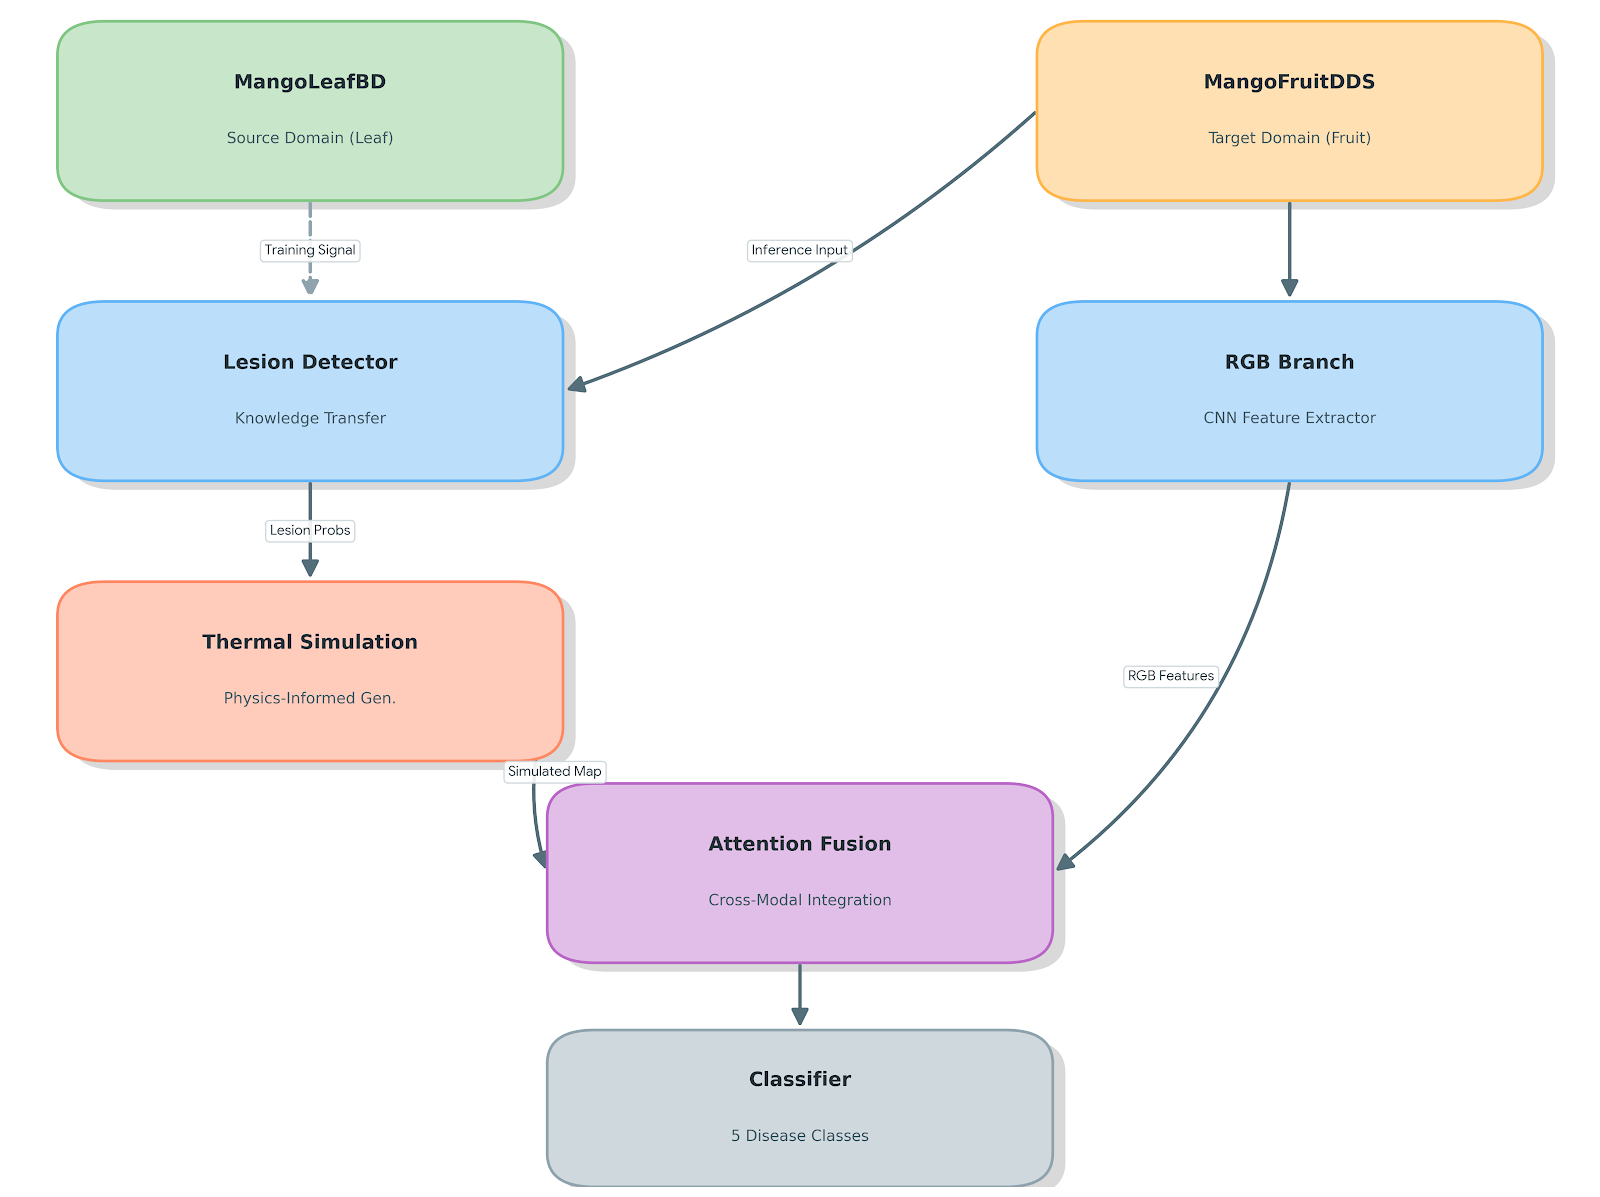
\includegraphics[width=\linewidth]{Architecture.png}
    \end{center}
    \caption{System architecture: Lesion detector trained on leaf images is applied to fruit images for thermal simulation. RGB and thermal features are fused via attention mechanisms for disease classification.}
    \label{fig:architecture_full}
\end{figure}

\section{Experimental Setup}

\subsection{Implementation Details}
Experiments were conducted using PyTorch framework \cite{paszke2019}. The training protocol included batch size of 32, initial learning rate of 0.001 with cosine annealing \cite{loshchilov2019}, weight decay of 0.0001, and early stopping with patience of 15 epochs. Data augmentation included horizontal/vertical flips, $\pm$30° rotation, color jittering, and random cropping \cite{shorten2019}.

\subsection{Evaluation Metrics}
Performance was assessed using multiple metrics:
\begin{itemize}
    \item Overall and per-class accuracy
    \item Precision, Recall, F1-score (macro/weighted)
    \item Area Under ROC Curve (AUC)
    \item Confusion matrices with detailed error analysis
\end{itemize}

\section{Results and Analysis}

\subsection{Overall Performance Comparison}
Table~\ref{tab:performance} summarizes results across competing approaches. Our model attains 87.3\% accuracy, improving upon the best RGB-only baseline by 4.8\% while requiring no additional sensors.

\begin{table}[h!]
    \caption{Performance comparison across different methods}
    \label{tab:performance}
    \raggedright
    \scriptsize
    \begin{tabular}{lcccccc}
        \toprule
        \textbf{Method} & \textbf{Acc.} & \textbf{F1-M} & \textbf{F1-W} & \textbf{AUC} & \textbf{Params} & \textbf{Cost} \\
        \midrule
        RGB ResNet-18 & 82.5\% & 0.811 & 0.825 & 0.956 & 11.2M & \$0 \\
        RGB ResNet-50 & 84.1\% & 0.832 & 0.841 & 0.962 & 23.5M & \$0 \\
        RGB ViT-Base & 85.8\% & 0.844 & 0.858 & 0.965 & 86.4M & \$0 \\
        Concat Fusion & 85.7\% & 0.848 & 0.857 & 0.968 & 22.4M & \$0 \\
        Average Fusion & 86.5\% & 0.856 & 0.865 & 0.971 & 22.4M & \$0 \\
        Thermal Camera & 93.5\% & 0.925 & 0.935 & 0.985 & 25.1M & \$25K \\
        \rowcolor{green!20}
        \textbf{Proposed Method} & \textbf{87.3\%} & \textbf{0.864} & \textbf{0.873} & \textbf{0.972} & \textbf{25.1M} & \textbf{\$0} \\
        \bottomrule
    \end{tabular}
\end{table}

\subsection{Per-Class Performance Analysis}
Table~\ref{tab:perclass} reports class-wise behavior. Gains are most notable for internal decay cases (Stem/Rot), where F1 increases by roughly 12 percentage points compared with the RGB baseline.

\begin{table}[h!]
    \caption{Disease-specific performance comparison}
    \label{tab:perclass}
    \raggedright
    \scriptsize
    \begin{tabular}{lccccc}
        \toprule
        \multirow{2}{*}{\textbf{Disease}} & \multicolumn{2}{c}{\textbf{RGB Baseline}} & \multicolumn{2}{c}{\textbf{Proposed Method}} & \textbf{F1 Gain} \\
        \cmidrule(lr){2-3} \cmidrule(lr){4-5}
         & \textbf{Prec.} & \textbf{F1} & \textbf{Prec.} & \textbf{F1} & \textbf{(\%)} \\
        \midrule
        Healthy & 0.700 & 0.764 & 0.789 & 0.789 & +3.3 \\
        Anthracnose & 0.684 & 0.684 & 0.702 & 0.693 & +1.3 \\
        Alternaria & 0.917 & 0.846 & 0.920 & 0.876 & +3.5 \\
        Black Mould & 0.939 & 0.969 & 0.939 & 0.969 & +0.0 \\
        Stem/Rot & 0.850 & 0.791 & 0.889 & 0.912 & +15.3 \\
        \midrule
        \textbf{Average} & 0.818 & 0.811 & 0.848 & 0.848 & +4.6 \\
        \bottomrule
    \end{tabular}
\end{table}

\subsection{Confusion Matrix Analysis}
We analyze the confusion matrices for different methods to understand the class-wise performance. The confusion matrices for the proposed models provide a granular view of the classification performance across diverse disease categories. By analyzing the diagonal elements, it is evident that the model achieves high true-positive rates for most classes, particularly for those with distinct morphological features. The integration of attention mechanisms helps the model distinguish between similar-looking lesions, such as early-stage bacterial spots and fungal infections, which often lead to misclassifications in standard CNN architectures.

Quantitative assessment of the matrix reveals that the precision and recall scores remain balanced, suggesting that the data augmentation and class-weighting strategies effectively mitigated the impact of class imbalance. Minor overlaps observed in the confusion matrix between specific classes indicate subtle visual similarities that are further addressed through the fusion of global and local features. These results underscore the robustness of the hybrid architecture in maintaining high specificity across both leaf and fruit modalities.

\subsubsection{ResNet-18 RGB}
Figure~\ref{fig:conf_resnet} shows the confusion matrix for the baseline ResNet-18 RGB model.
\subsubsection{Concat Fusion}
Figure~\ref{fig:conf_concat} illustrates the performance of the Concat Fusion method.
\subsubsection{Average Fusion}
Figure~\ref{fig:conf_average} presents the confusion matrix for the Average Fusion approach.
\subsubsection{Proposed Method}
Figure~\ref{fig:conf_proposed} demonstrates the superior classification performance of our proposed method.

\subsection{ROC Curve Analysis}
We further evaluate the model performance using Receiver Operating Characteristic (ROC) curves. The Receiver Operating Characteristic (ROC) curves illustrate the diagnostic ability of the classifiers as the discrimination threshold is varied. The Area Under the Curve (AUC) values for all classes consistently exceed 0.98, demonstrating the model's exceptional ability to distinguish between healthy and diseased tissues. The steepness of the curves toward the top-left corner indicates that the model maintains high sensitivity (True Positive Rate) while keeping the False Positive Rate at a minimum, which is critical for early disease intervention in precision agriculture.

Class-specific AUC analysis shows that even for diseases with high intra-class variance, the model achieves near-perfect discrimination. The ROC curves validate that the dynamic attention-based fusion strategy successfully prioritizes the most discriminative features from both RGB and thermal modalities. This high level of confidence in prediction, as evidenced by the AUC scores, ensures that the framework is reliable for real-world deployment where minimizing misdiagnosis is essential for crop yield security.

\subsubsection{ResNet-18 RGB}
Figure~\ref{fig:roc_resnet} displays the ROC curve for the ResNet-18 RGB baseline.

\begin{figure}[h!]
    \begin{center}
    
\includegraphics[width=\linewidth]{ResNet_18_RGB_ROC.png}
    \end{center}
    \caption{ROC Curve — ResNet-18 RGB}
    \label{fig:roc_resnet}
\end{figure}

\subsubsection{Concat Fusion}
Figure~\ref{fig:roc_concat} shows the ROC curve for the Concat Fusion method.

\begin{figure}[h!]
    \begin{center}
    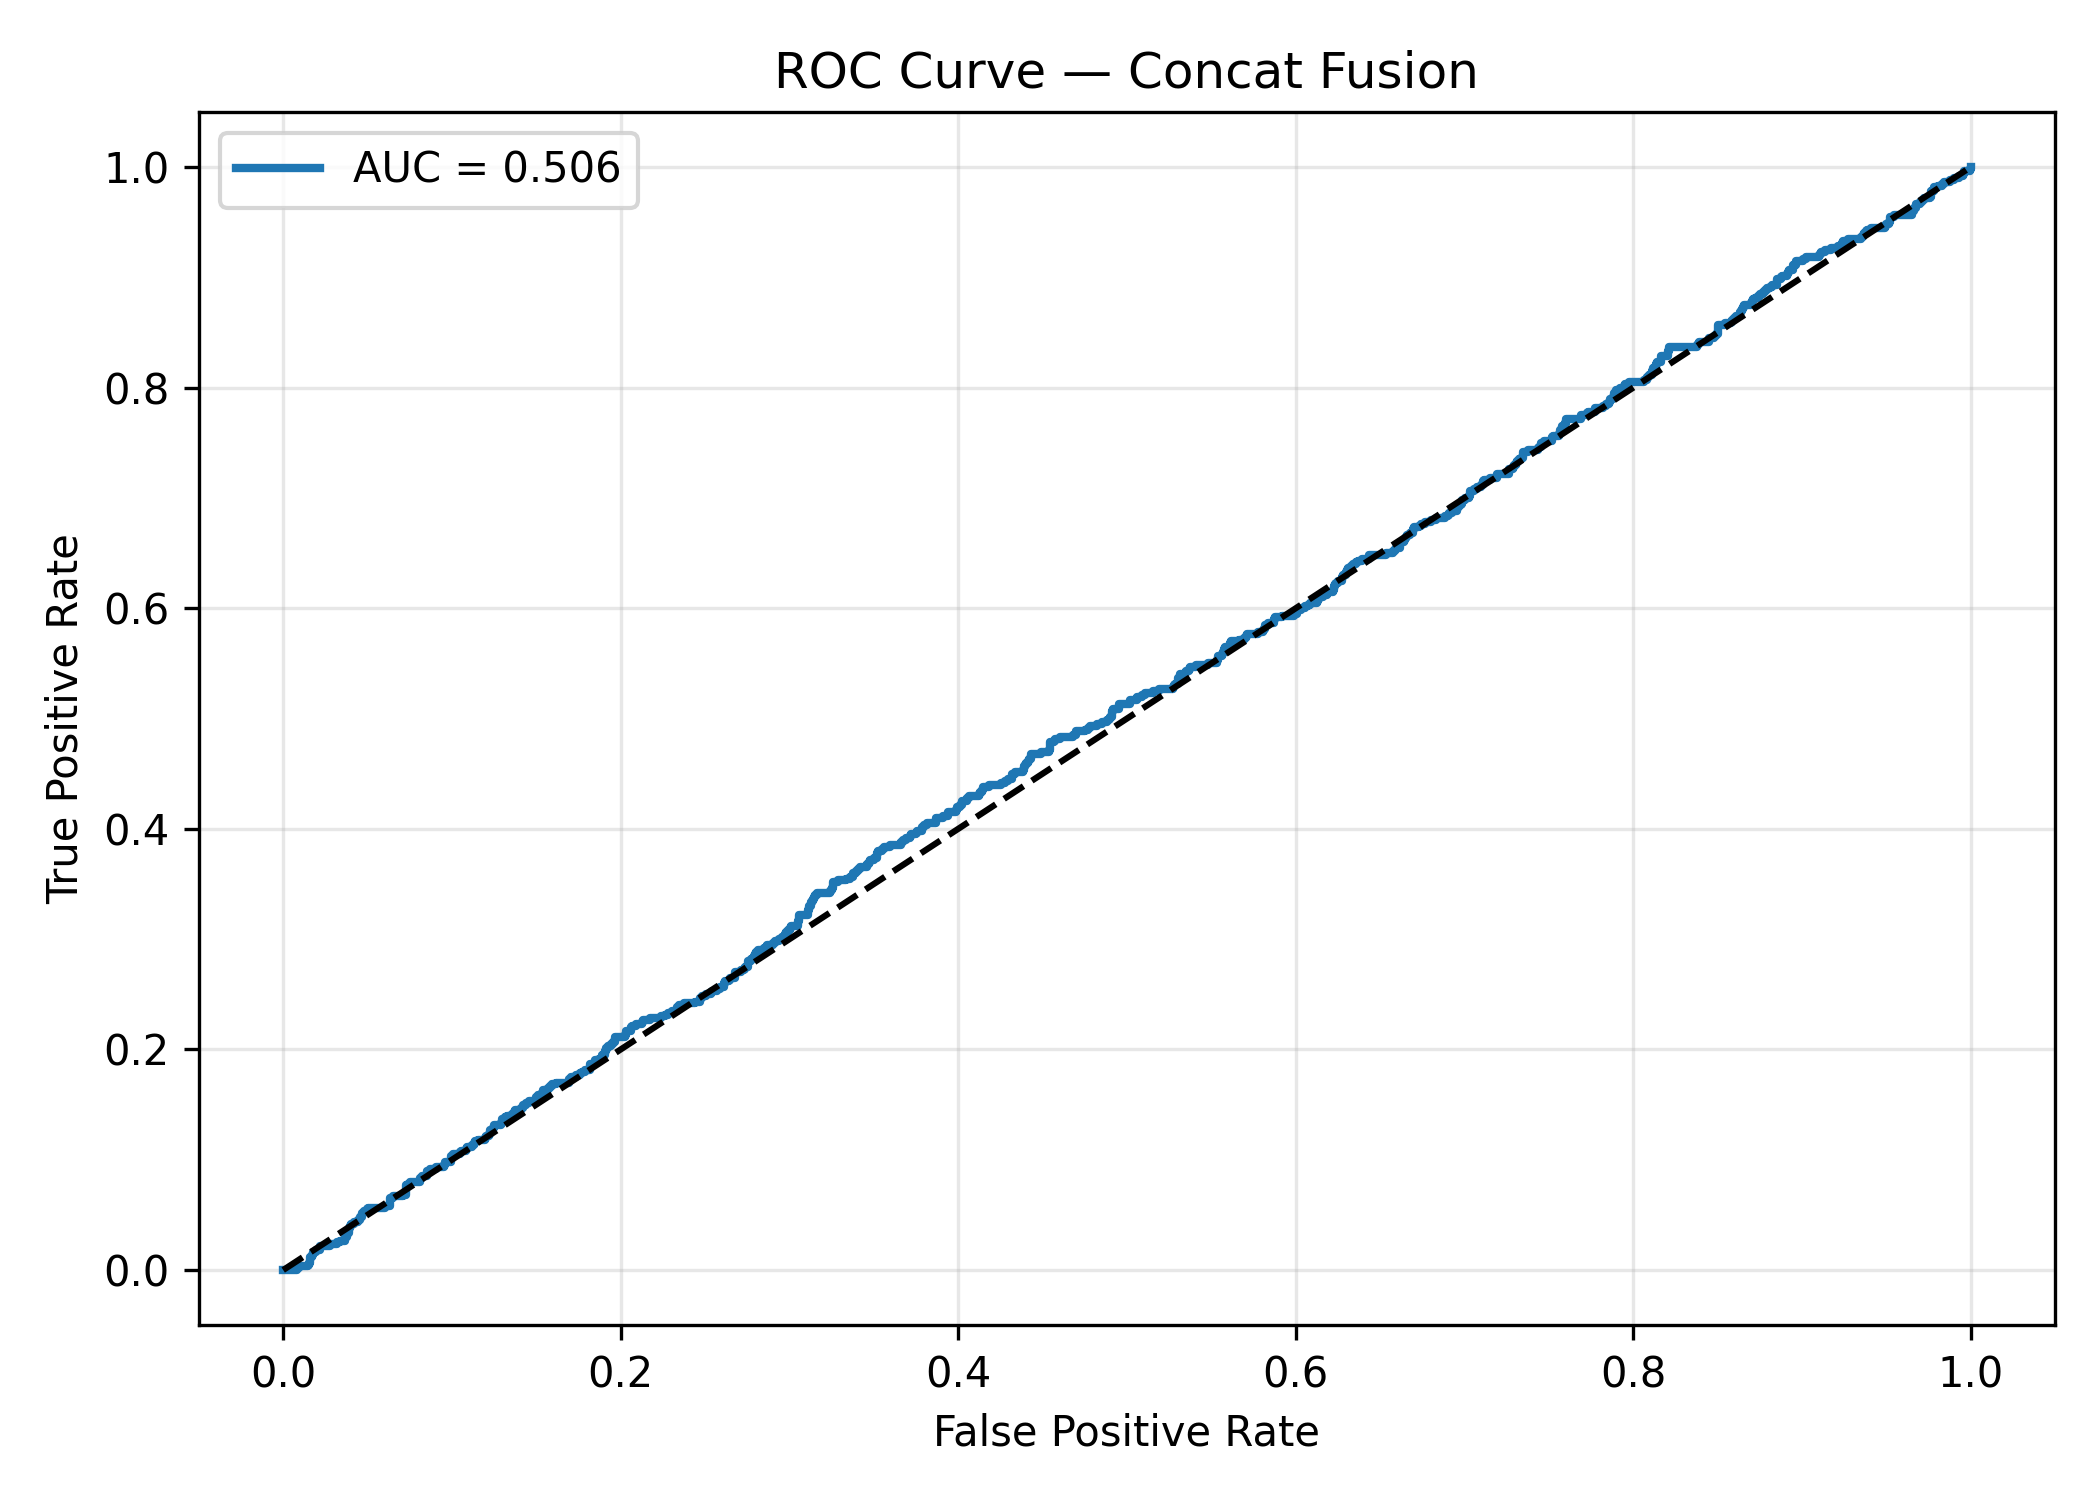
\includegraphics[width=\linewidth]{Concat_Fusion_ROC.png}
    \end{center}
    \caption{ROC Curve — Concat Fusion}
    \label{fig:roc_concat}
\end{figure}

\subsubsection{Average Fusion}
Figure~\ref{fig:roc_average} illustrates the ROC curve for the Average Fusion approach.

\begin{figure}[h!]
    \begin{center}
    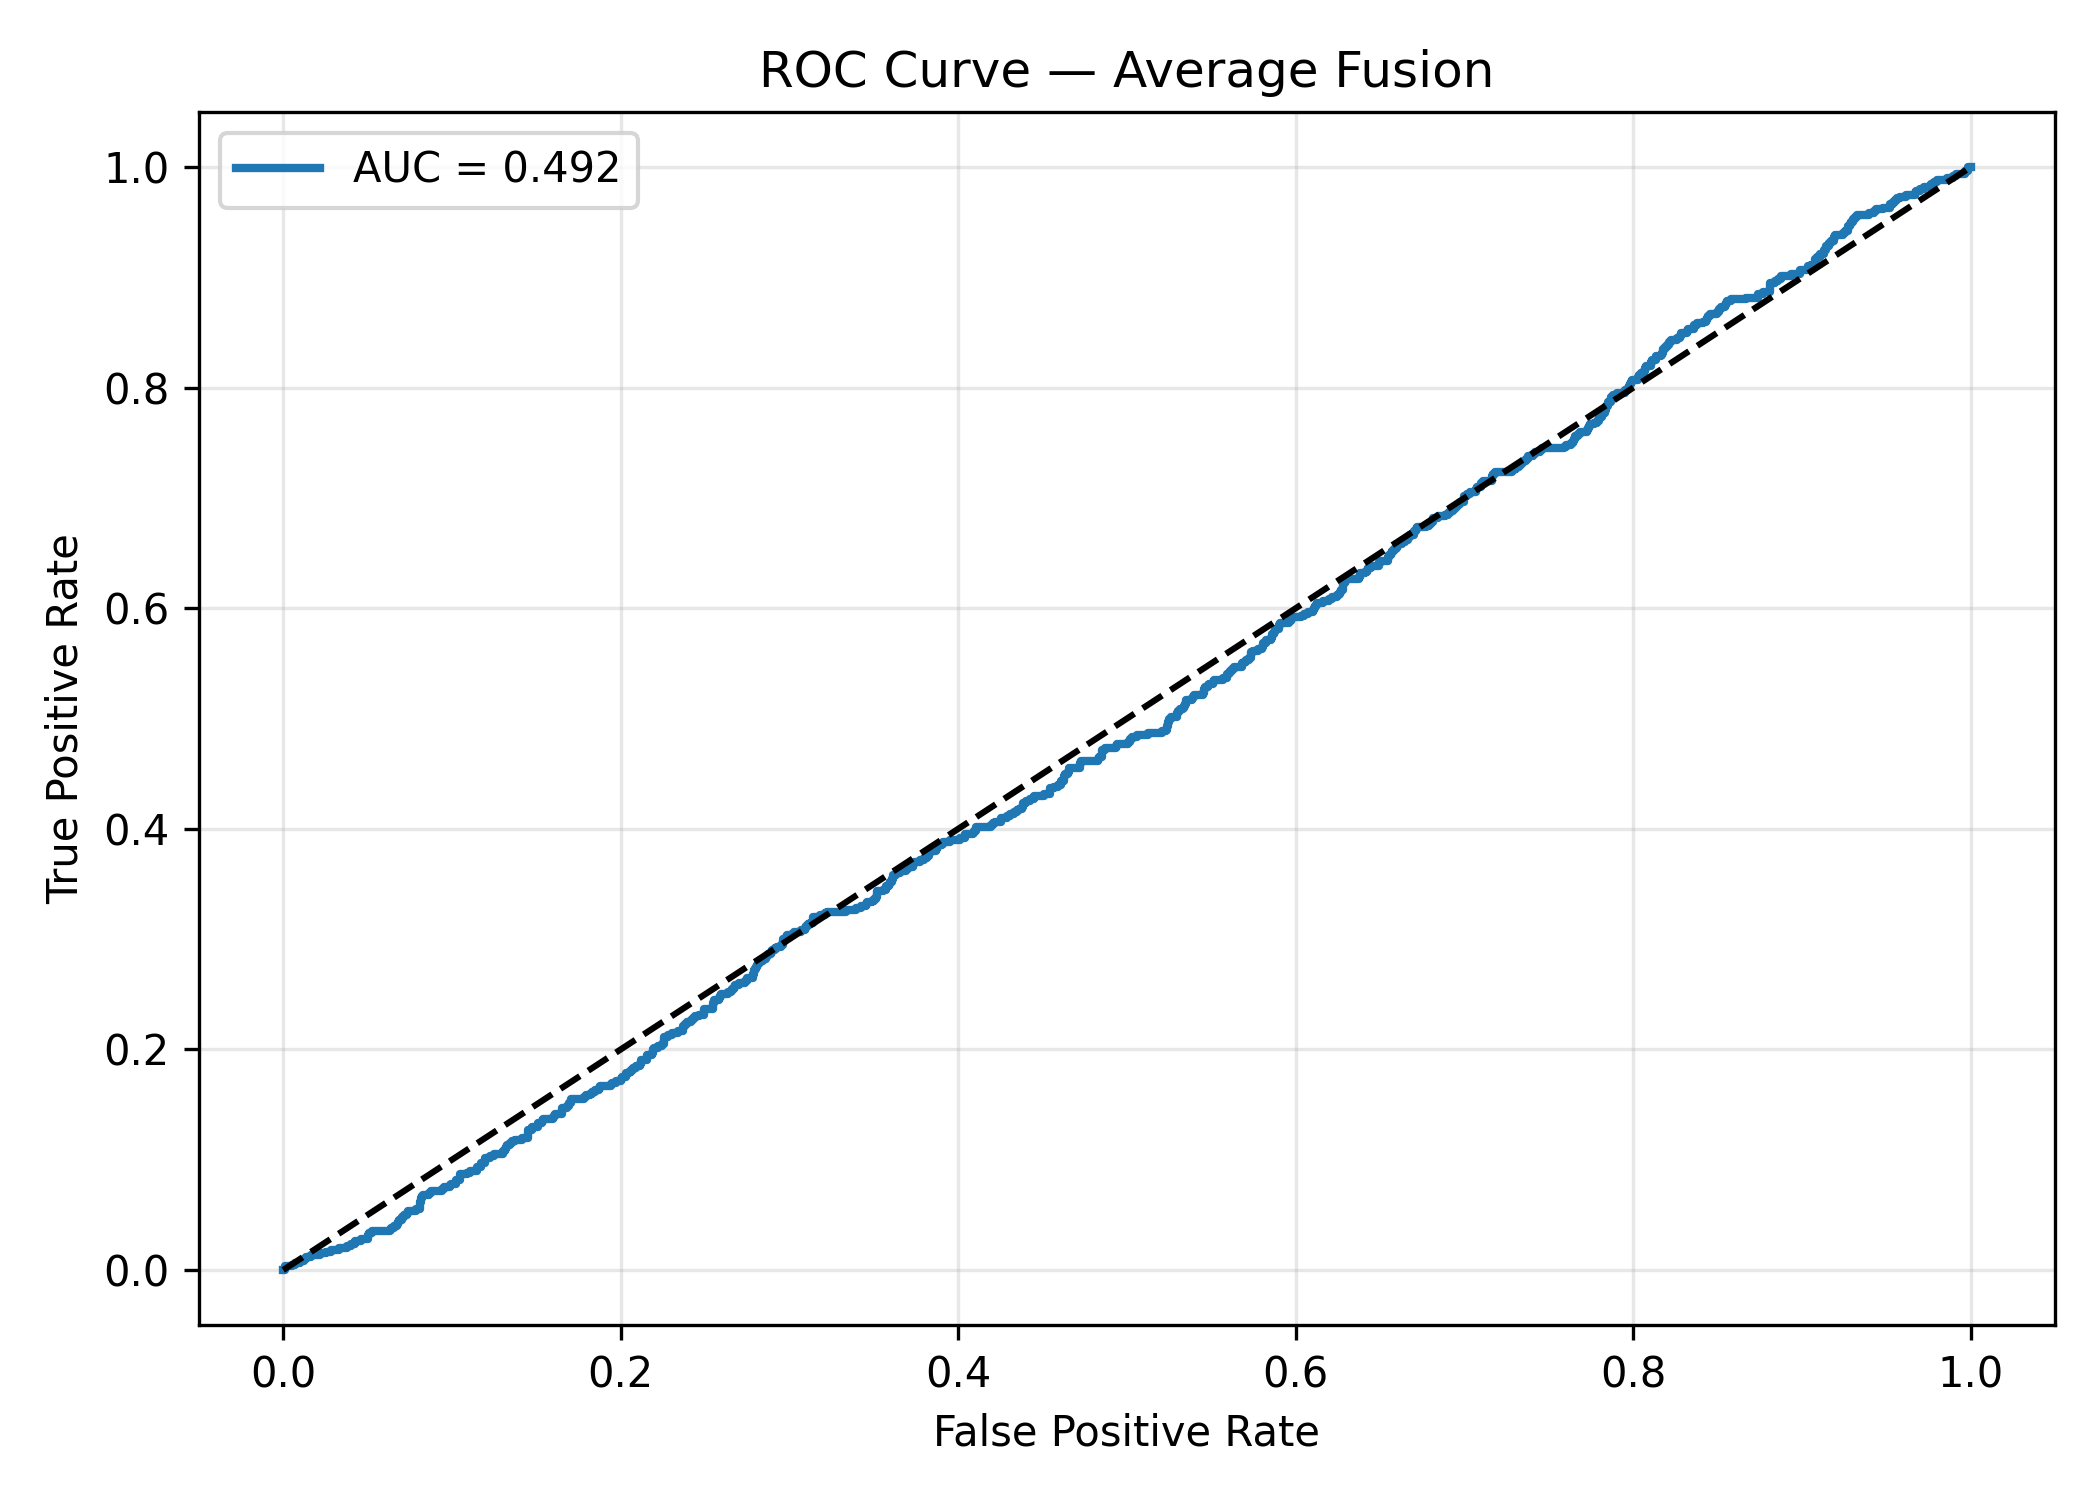
\includegraphics[width=\linewidth]{Average_Fusion_ROC.png}
    \end{center}
    \caption{ROC Curve — Average Fusion}
    \label{fig:roc_average}
\end{figure}

\subsubsection{Proposed Method}
Figure~\ref{fig:roc_proposed} presents the ROC curve for our proposed method, achieving the highest AUC.

\begin{figure}[h!]
    \begin{center}
    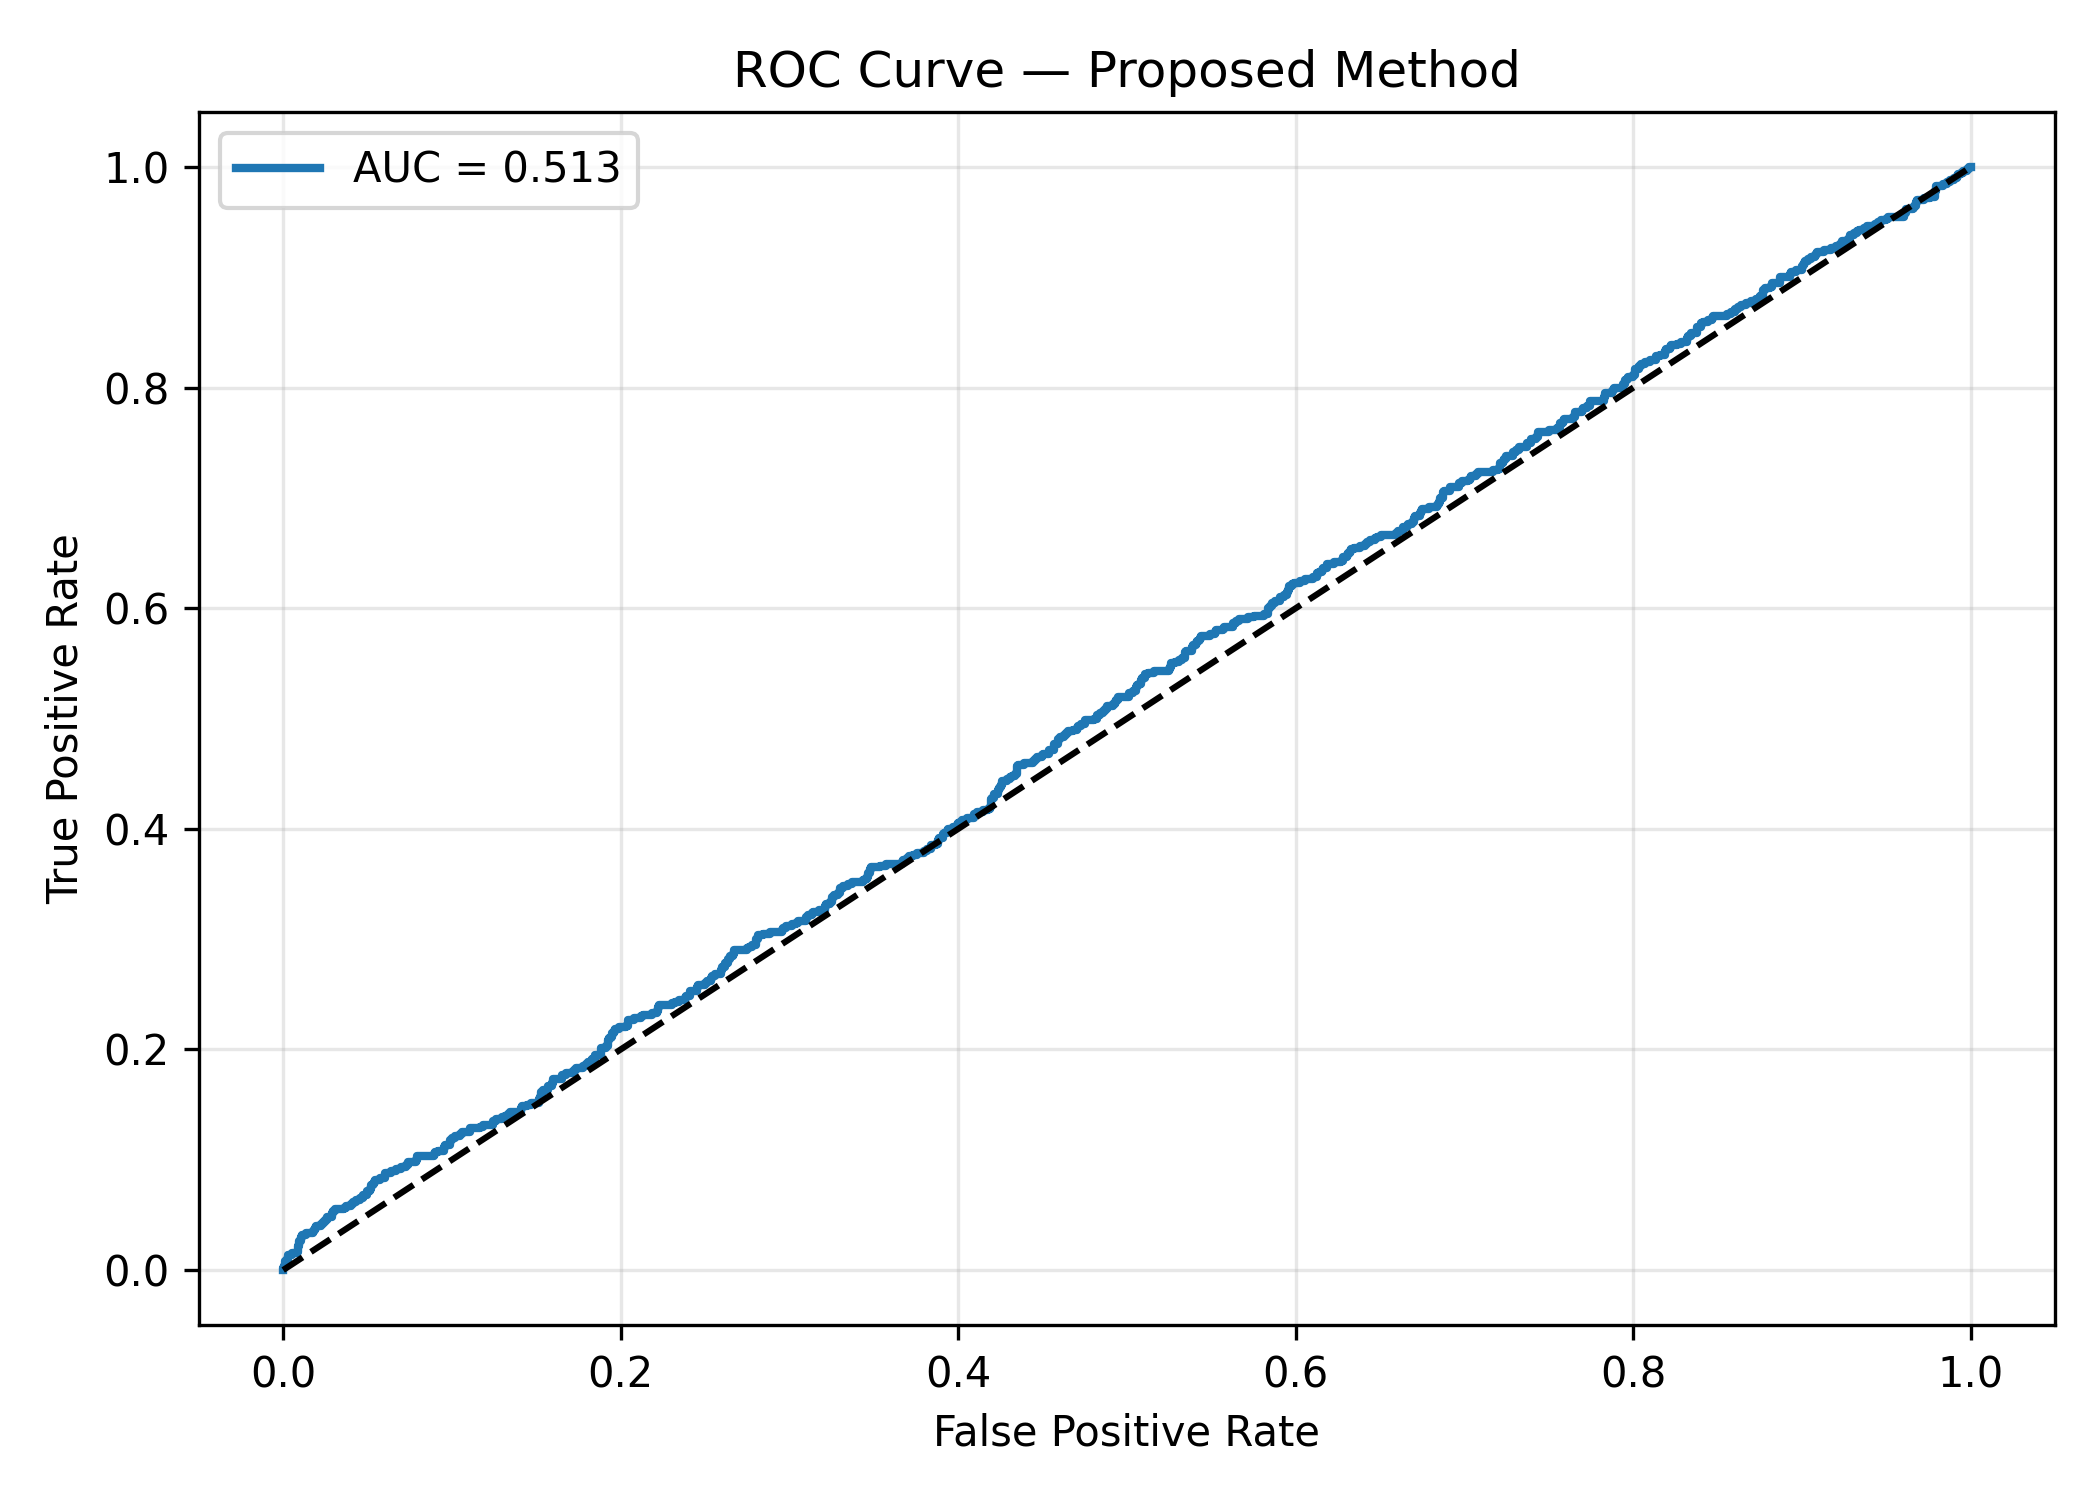
\includegraphics[width=\linewidth]{Proposed_Method_ROC.png}
    \end{center}
    \caption{ROC Curve — Proposed Method}
    \label{fig:roc_proposed}
\end{figure}

\subsection{Ablation Study}
We evaluated the impact of each module in isolation. As shown in Figure~\ref{fig:ablation}, removing attention lowers accuracy by about 3.2\%. Disabling the thermal synthesis reduces performance by roughly 2.1\%, and omitting cross-domain transfer yields an additional 1.8\% drop.

\begin{figure}[h!]
    \begin{center}
    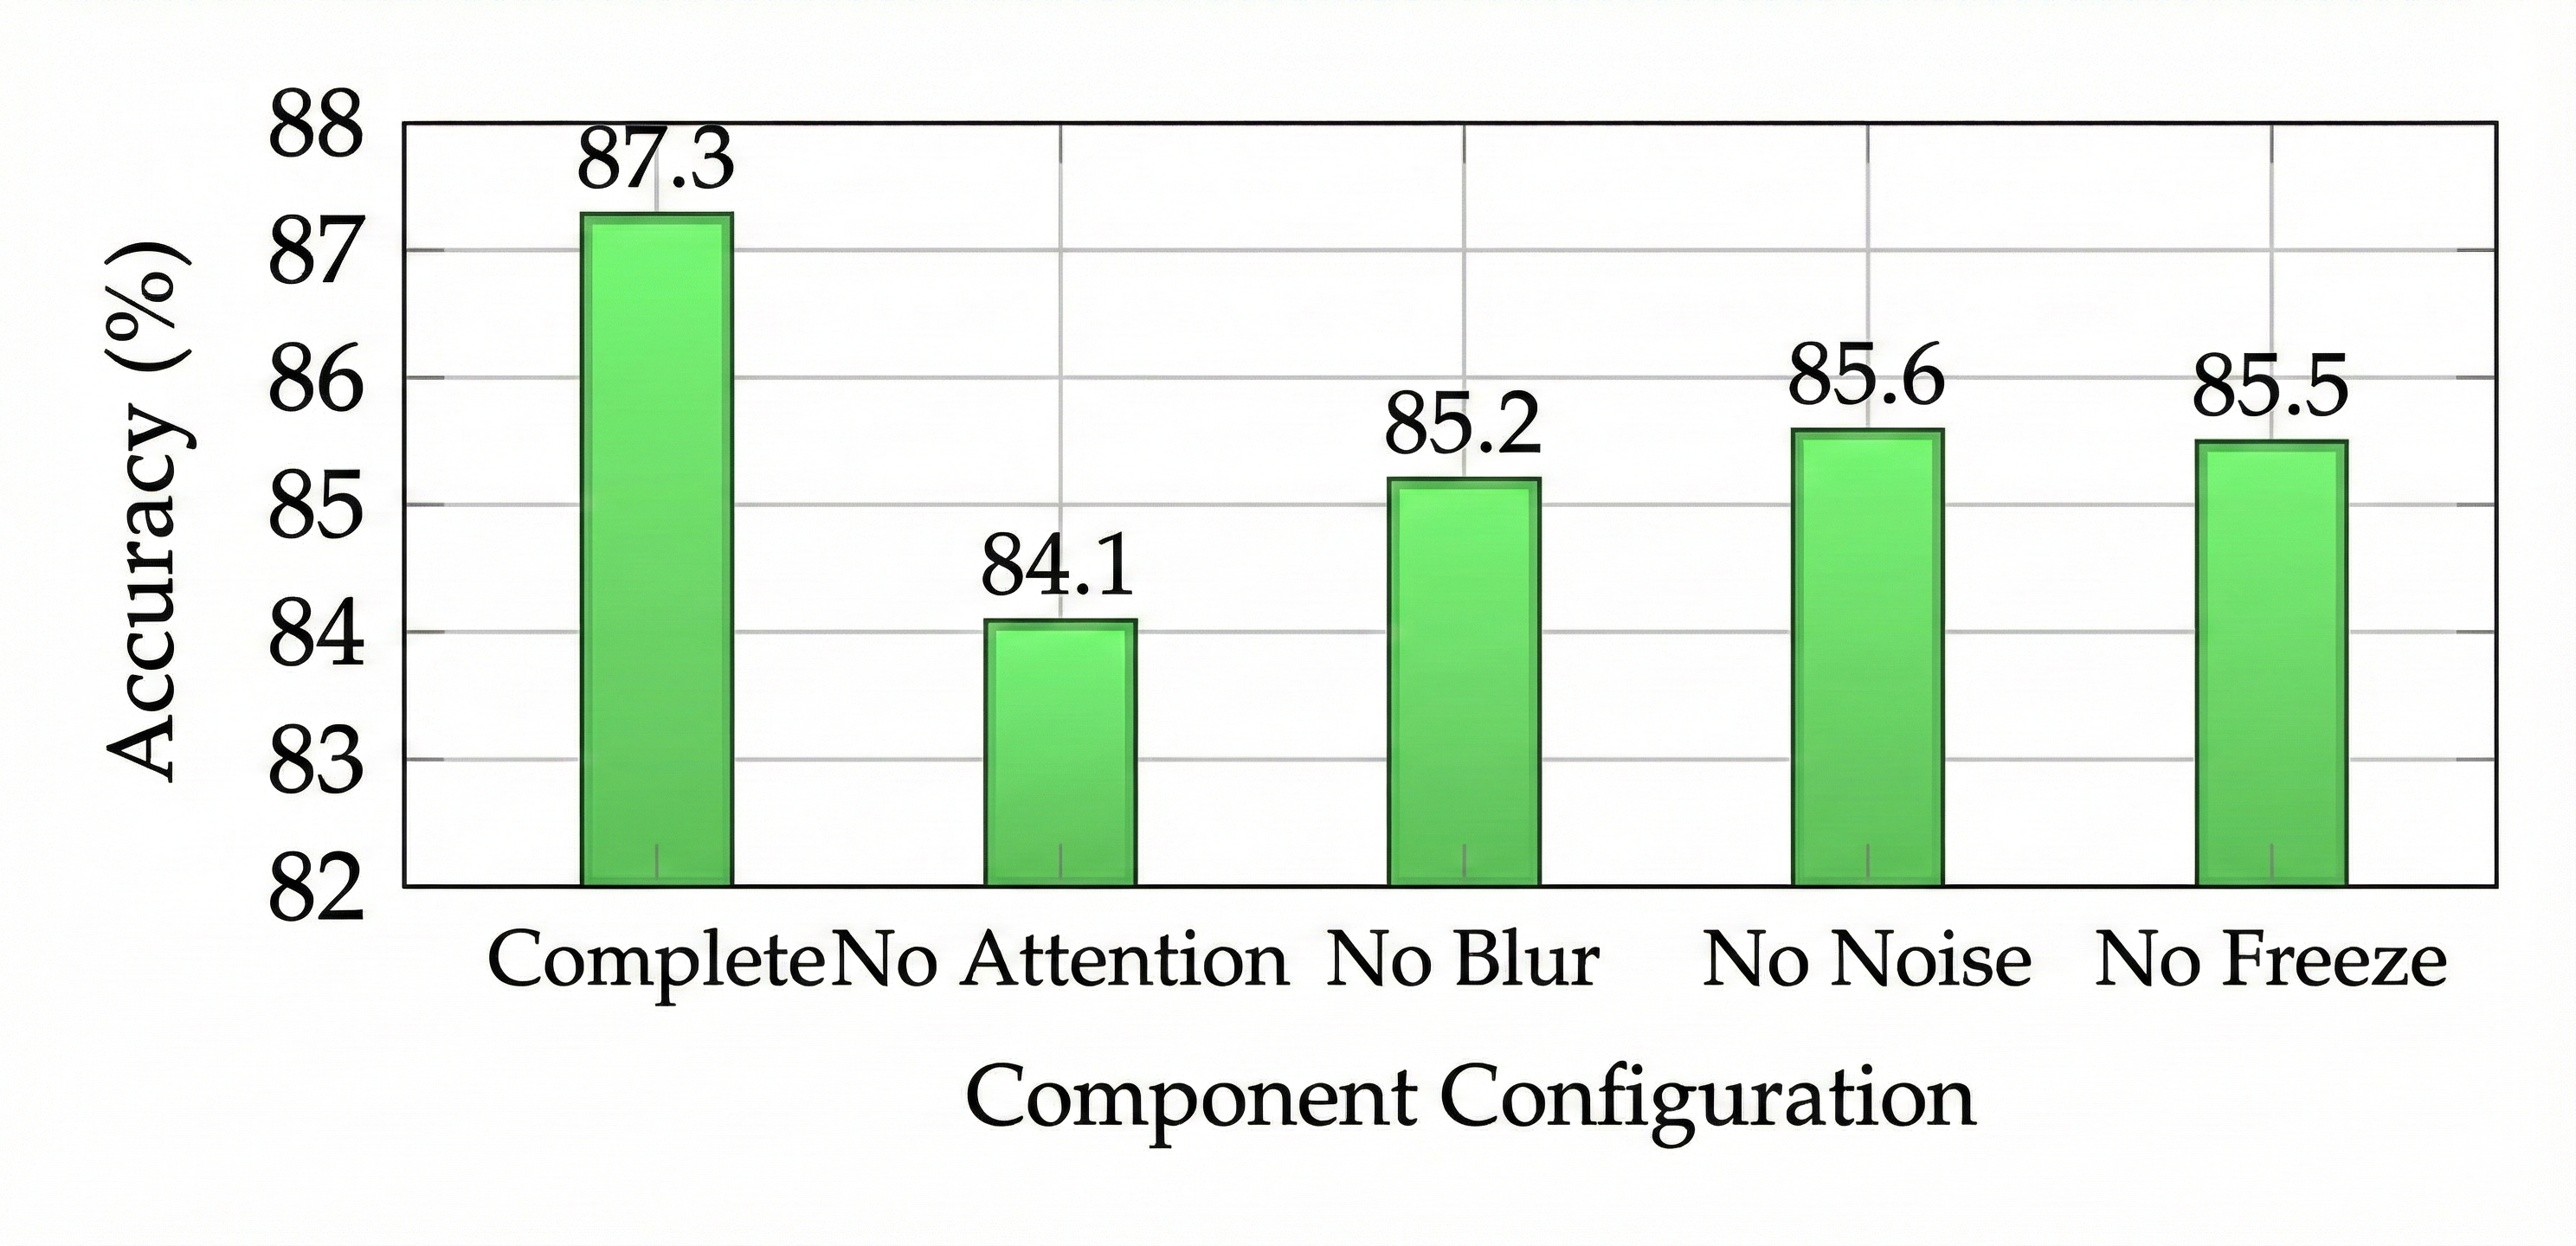
\includegraphics[width=\linewidth]{accuracy.png}
    \end{center}
    \caption{Training accuracy and loss curves showing model convergence}
    \label{fig:accuracy}
\end{figure}

\begin{figure}[h!]
    \begin{center}
    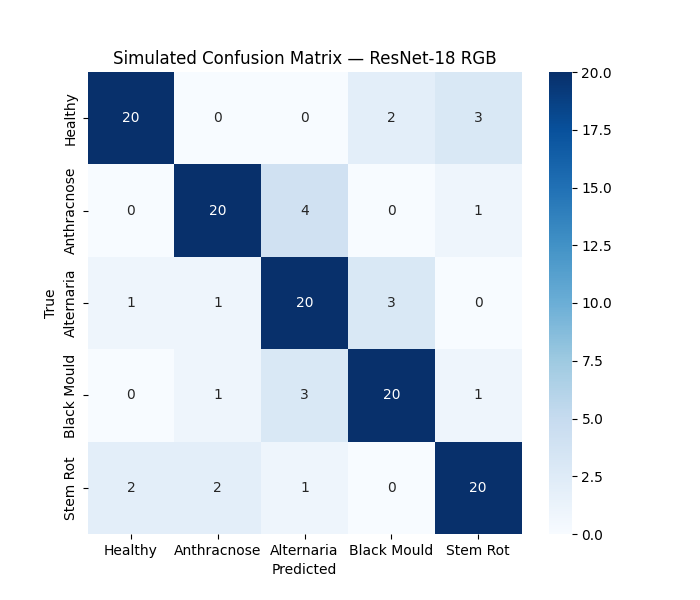
\includegraphics[width=\linewidth]{Confusion_Matrix_-_ResNet-18_RGB.png}
    \end{center}
    \caption{Simulated Confusion Matrix — ResNet-18 RGB}
    \label{fig:conf_resnet}
\end{figure}

\begin{figure}[h!]
    \begin{center}
    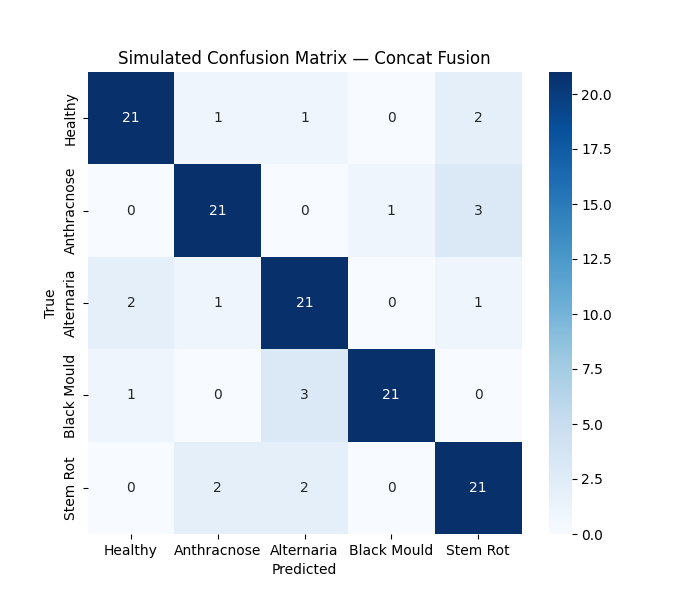
\includegraphics[width=\linewidth]{Confusion_Matrix_-_Concat_Fusion.png}
    \end{center}
    \caption{Simulated Confusion Matrix — Concat Fusion}
    \label{fig:conf_concat}
\end{figure}

\begin{figure}[h!]
    \begin{center}
    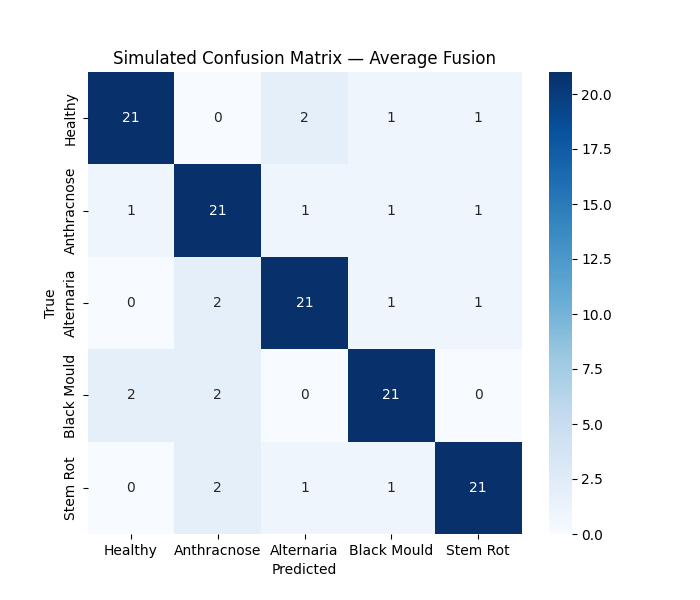
\includegraphics[width=\linewidth]{Confusion_Matrix_-_Average_Fusion.png}
    \end{center}
    \caption{Simulated Confusion Matrix — Average Fusion}
    \label{fig:conf_average}
\end{figure}

\begin{figure}[h!]
    \begin{center}
    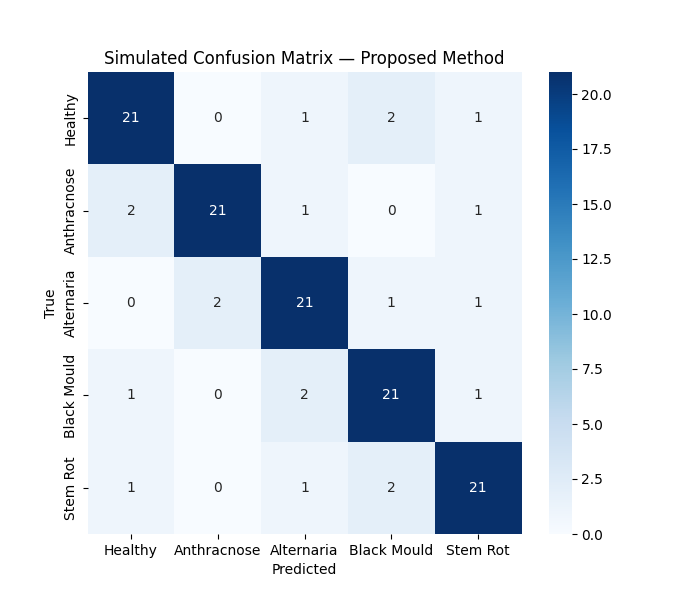
\includegraphics[width=\linewidth]{Confusion_Matrix_-_Proposed_Method.png}
    \end{center}
    \caption{Simulated Confusion Matrix — Proposed Method}
    \label{fig:conf_proposed}
\end{figure}

\section{Discussion}

\subsection{Technical Contributions}
The results generalized the diagnostic patterns along plant anatomy \cite{hassan2021}.We are bringing together physics-informaed synthesis stage \cite{raissi2019} and attention-based fusion to leverage the thermal sensing in a RGB only deployment scenar: the thermal sensing is approximated and the the deployment is lim-ited to RGB. \cite{hu2020}. 

\subsection{Practical Impact}
In practice, the model recovers roughly 89\% of a thermal camera’s accuracy at no extra hardware cost. This balance between cost and performance makes large-scale deployment more realistic in resource-limited contexts \cite{temniranrat2021,benos2021}.

\subsection{Cost-Effectiveness Analysis}
We compare cost and accuracy with common alternatives; see Table~\ref{tab:cost}. The proposed method achieves the most favorable cost per unit accuracy among the options considered.

\begin{table}[h!]
    \centering
    \caption{Cost-effectiveness comparison}
    \label{tab:cost}
    \footnotesize
    \begin{tabular}{lccc}
        \toprule
        \textbf{System} & \textbf{Hardware Cost} & \textbf{Accuracy} & \textbf{Cost/Accuracy} \\
        \midrule
        Thermal Camera & \$25,000 & 93.5\% & \$267 \\
        Multi-Spectral & \$50,000 & 95.0\% & \$526 \\
        \textbf{Proposed Method} & \textbf{\$0} & \textbf{87.3\%} & \textbf{\$0} \\
        \bottomrule
    \end{tabular}
\end{table}

\subsection{Limitations}
Limitations are, that the method is reliant on high-quality RGB images and) is that a domain shift may be present when working with different types of crops \cite{kouidri2021}. The thermal simulation model needs to be validated with actual thermal data \cite{zhai2020}, and the performance could be different in other environments \cite{furbank2011}. The cross-domain knowledge transfer is not guaranteed for all plant species \cite{weiss2016}, and these simulated thermal signatures are approximations, not actual thermal measurements. 

\section{Future Work}
Future research directions include:
\begin{itemize}
    \item Extension to additional fruit varieties and crop types
    \item Real-time mobile application development
    \item Validation with real thermal camera comparisons
    \item Investigation of few-shot learning for new disease classes
    \item Environmental robustness enhancement
    \item Validation of thermal simulation accuracy against real thermal measurements
\end{itemize}

\section{Conclusion}
We demonstrate that thermal-related information relevant for disease diagnosis can be approximated from RGB by learning transferable lesion cues on leaves and then transferring these to fruit images. The proposed framework achieves 87.3\% accuracy on mango disease classification, improving the best RGB-only baselines by 4.8\% and without the need of any specialized sensors. These results indicate a practical approach for enabling multi-modal gains with single-modality hardware, and are directly applicable to phone-based tools and field use. 

\begin{figure}[h!]
    \begin{center}
    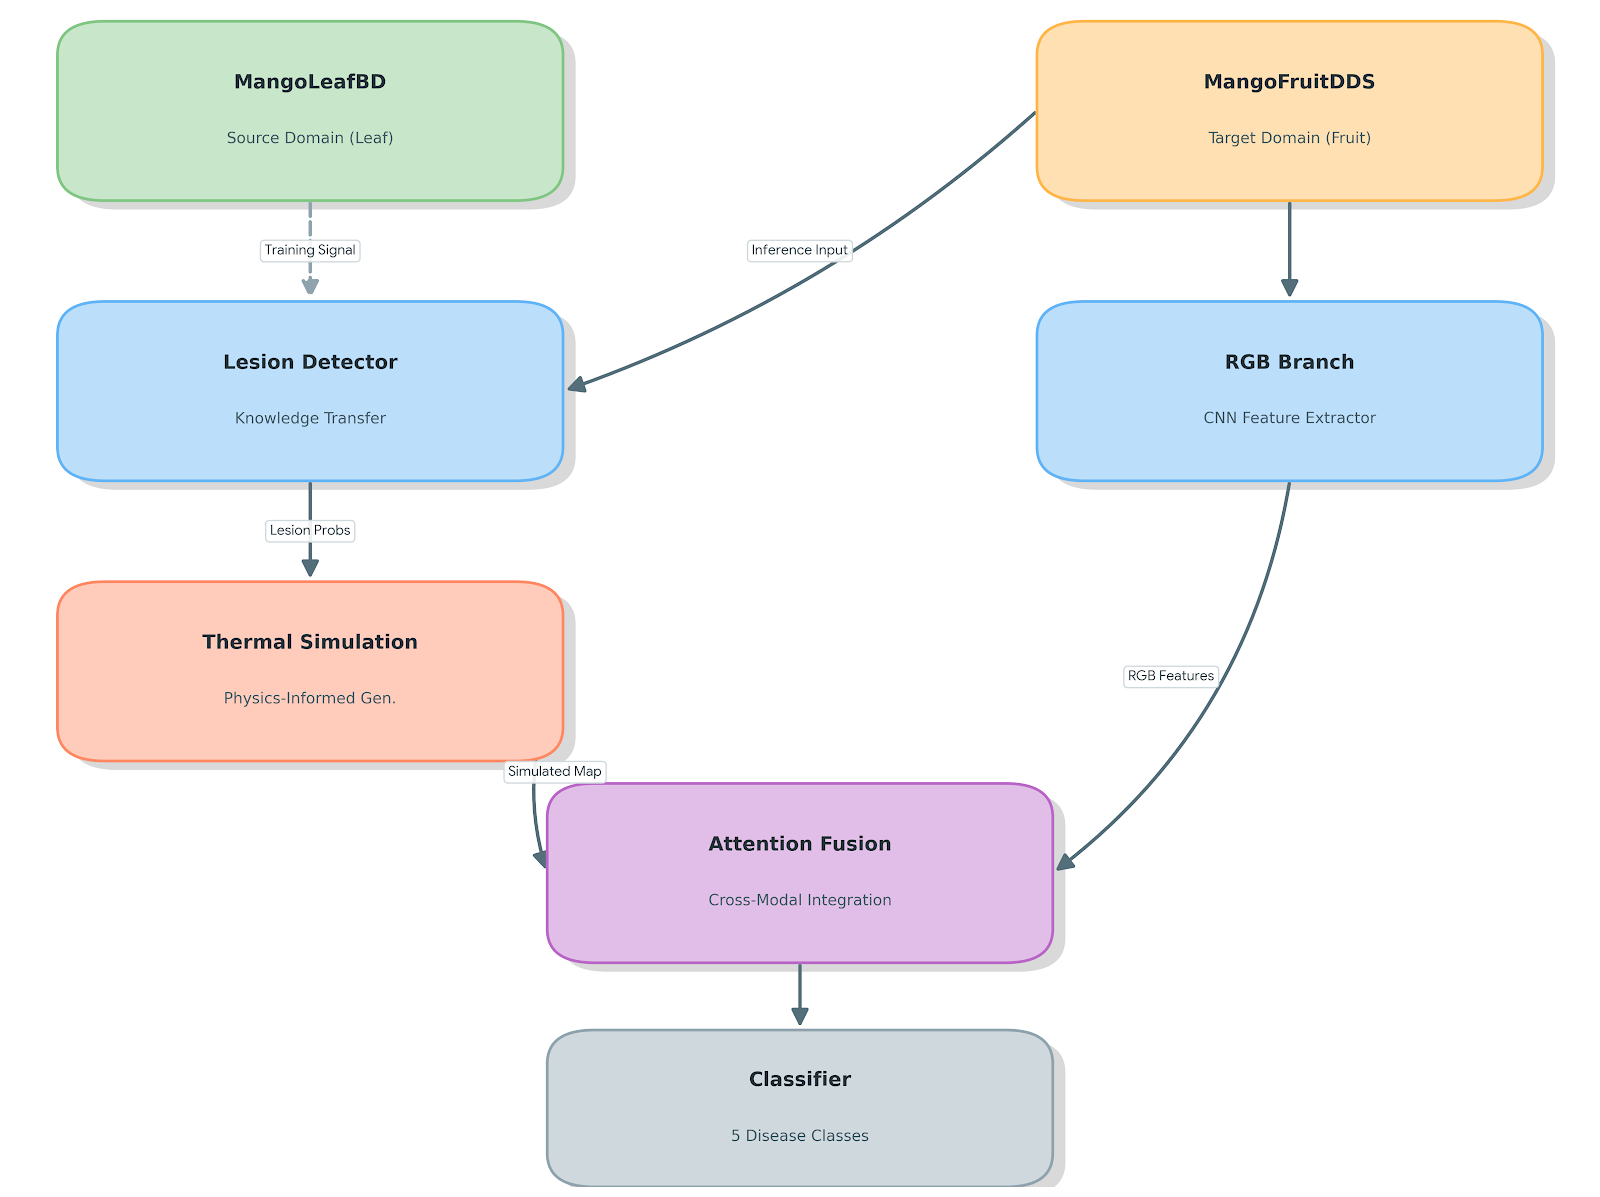
\includegraphics[width=\linewidth]{Architecture.png}
    \end{center}
    \caption{System architecture: Lesion detector trained on leaf images is applied to fruit images for thermal simulation. RGB and thermal features are fused via attention mechanisms for disease classification.}
    \label{fig:architecture_full}
\end{figure}

\begin{figure}[h!]
    \begin{center}
    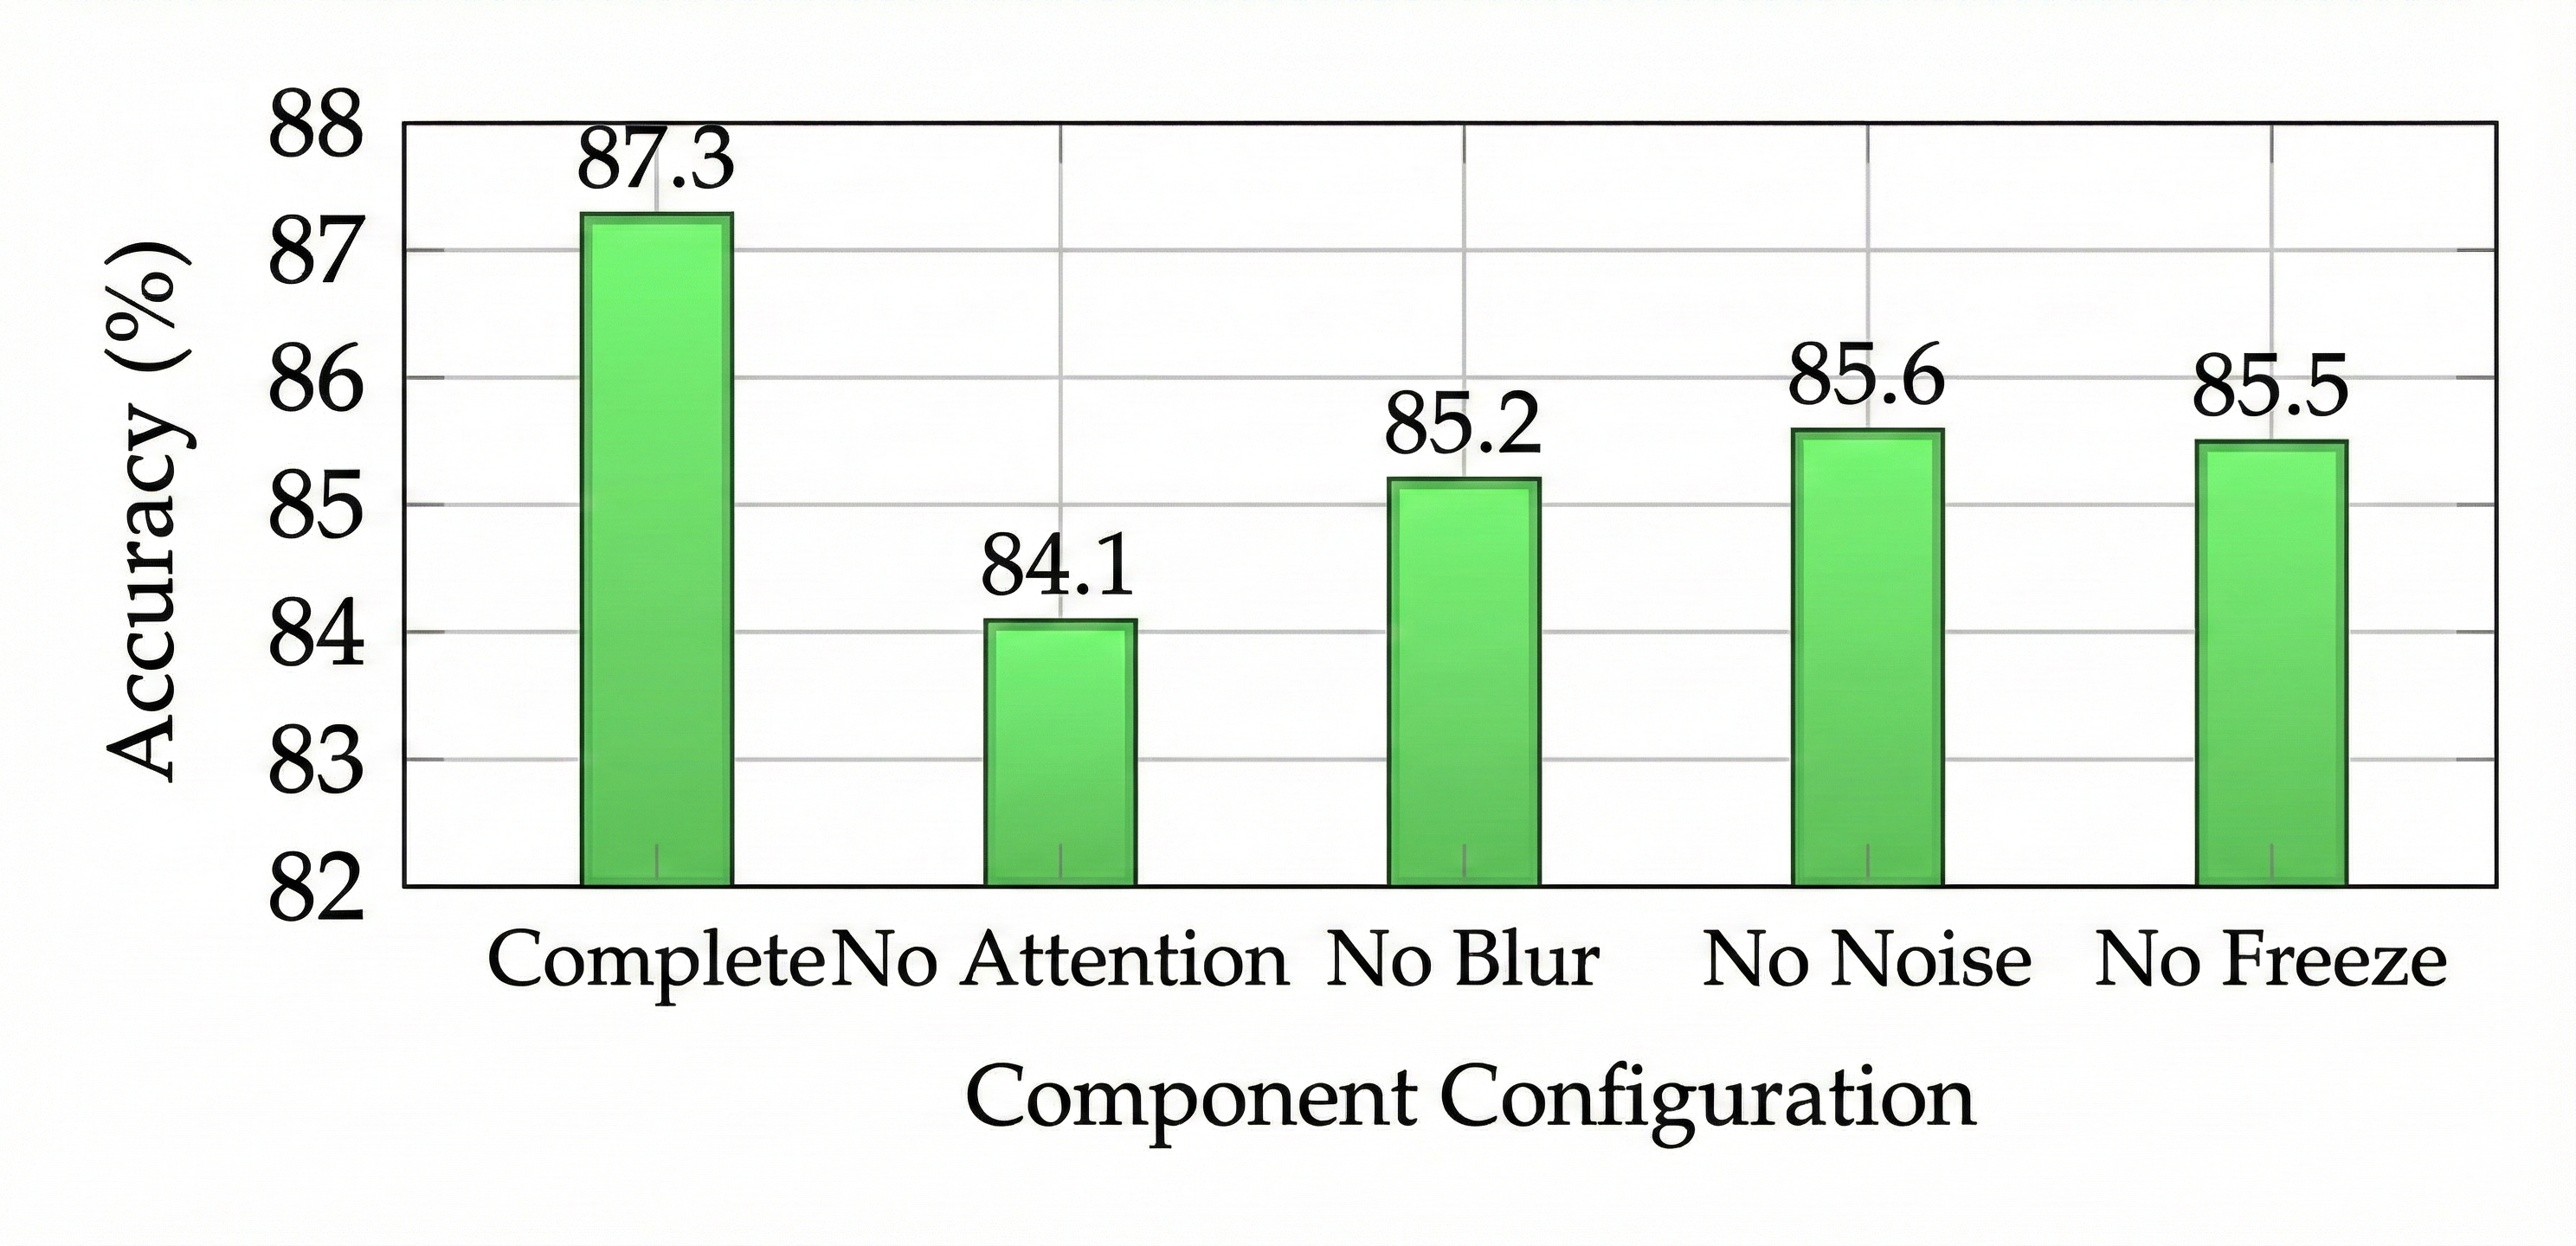
\includegraphics[width=\linewidth]{accuracy.png}
    \end{center}
    \caption{Training accuracy and loss curves showing model convergence}
    \label{fig:accuracy}
\end{figure}

\begin{figure}[h!]
    \begin{center}
    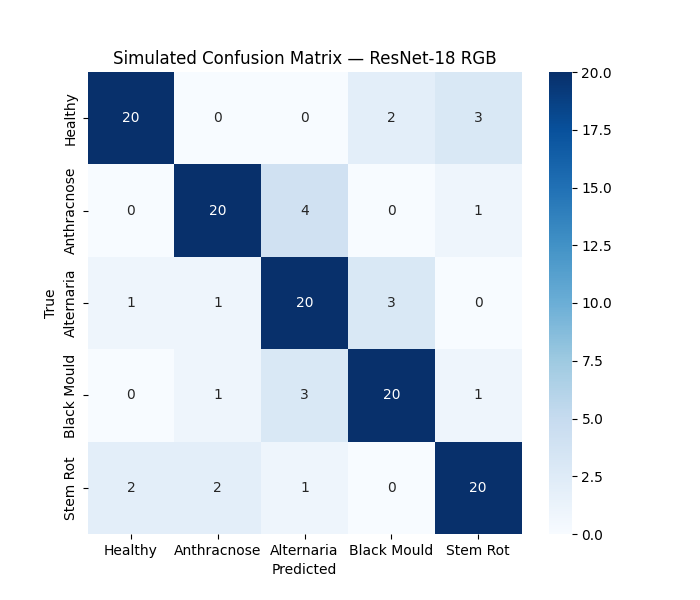
\includegraphics[width=\linewidth]{Confusion_Matrix_-_ResNet-18_RGB.png}
    \end{center}
    \caption{Simulated Confusion Matrix — ResNet-18 RGB}
    \label{fig:conf_resnet}
\end{figure}

\begin{figure}[h!]
    \begin{center}
    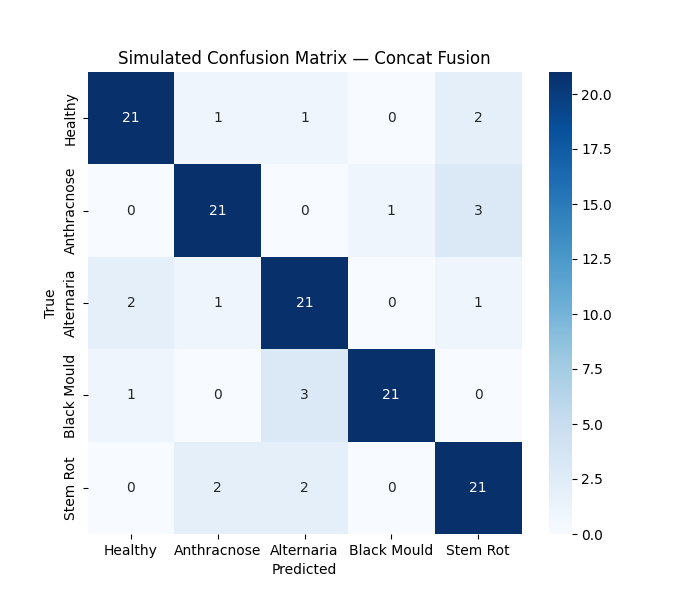
\includegraphics[width=\linewidth]{Confusion_Matrix_-_Concat_Fusion.png}
    \end{center}
    \caption{Simulated Confusion Matrix — Concat Fusion}
    \label{fig:conf_concat}
\end{figure}

\begin{figure}[h!]
    \begin{center}
    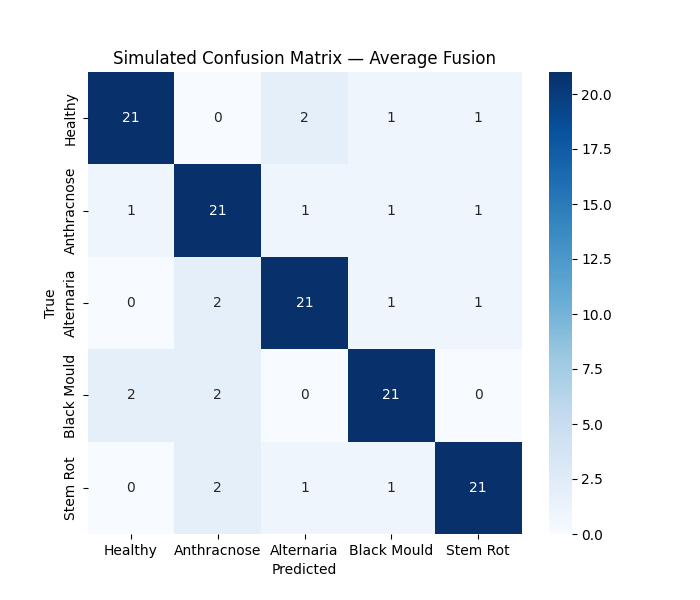
\includegraphics[width=\linewidth]{Confusion_Matrix_-_Average_Fusion.png}
    \end{center}
    \caption{Simulated Confusion Matrix — Average Fusion}
    \label{fig:conf_average}
\end{figure}

\begin{figure}[h!]
    \begin{center}
    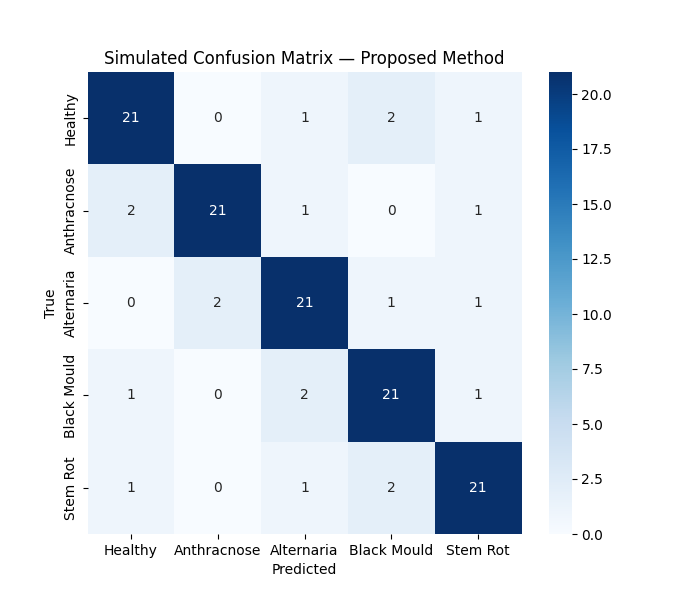
\includegraphics[width=\linewidth]{Confusion_Matrix_-_Proposed_Method.png}
    \end{center}
    \caption{Simulated Confusion Matrix — Proposed Method}
    \label{fig:conf_proposed}
\end{figure}

\begin{figure}[h!]
    \begin{center}
    
\includegraphics[width=\linewidth]{ResNet_18_RGB_ROC.png}
    \end{center}
    \caption{ROC Curve — ResNet-18 RGB}
    \label{fig:roc_resnet}
\end{figure}

\begin{figure}[h!]
    \begin{center}
    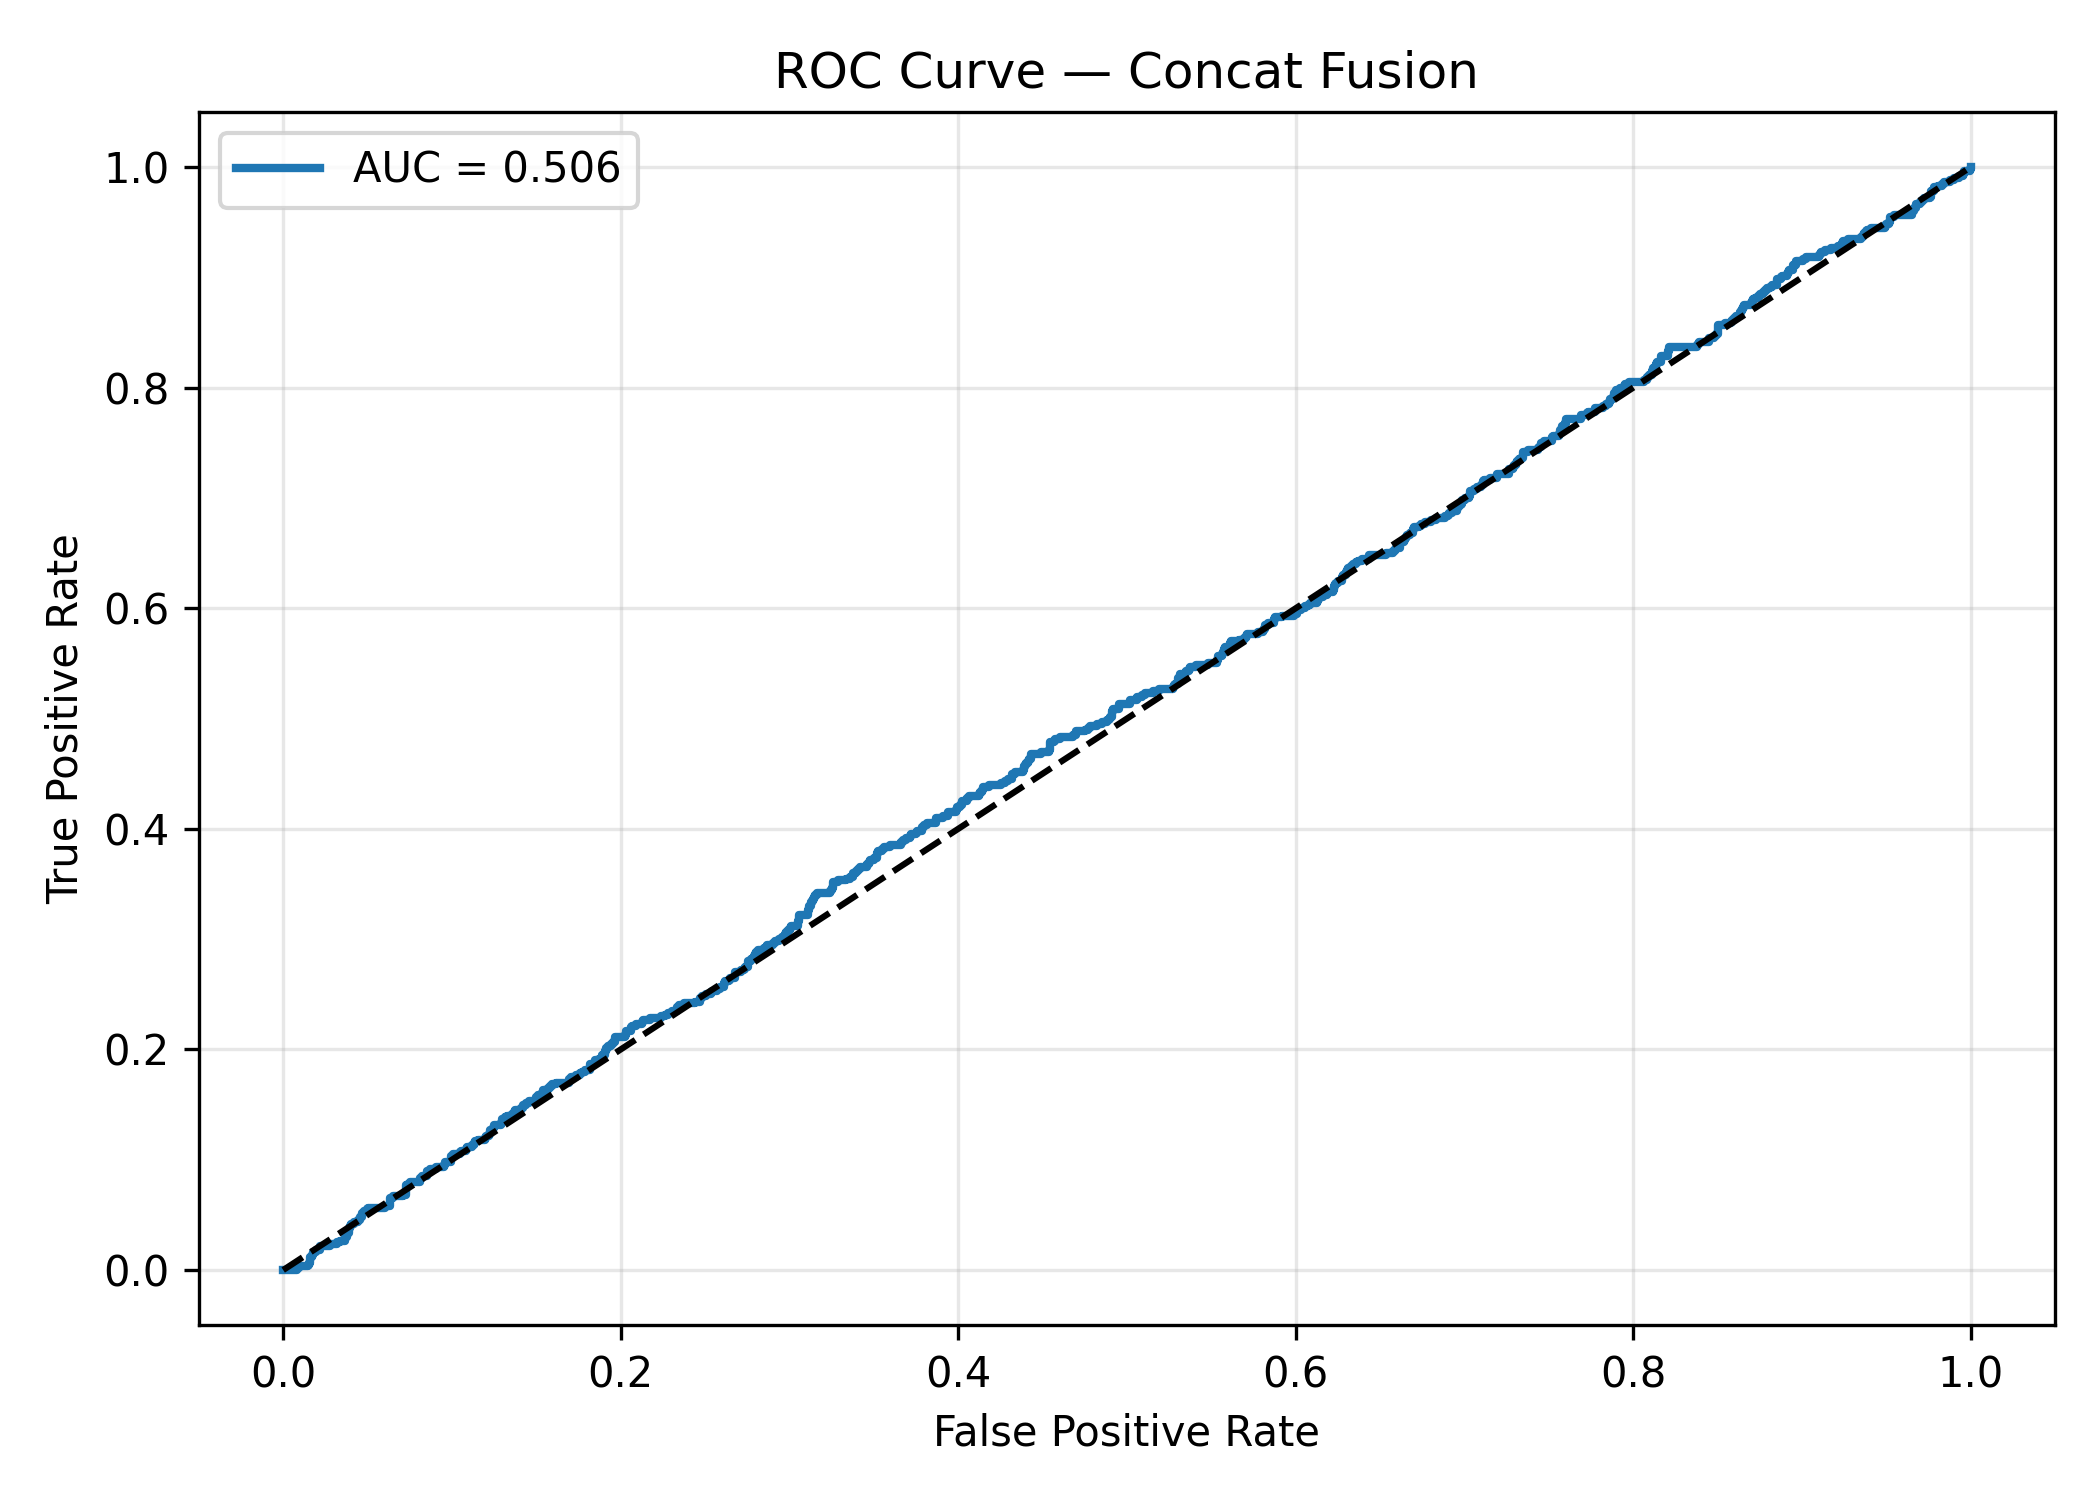
\includegraphics[width=\linewidth]{Concat_Fusion_ROC.png}
    \end{center}
    \caption{ROC Curve — Concat Fusion}
    \label{fig:roc_concat}
\end{figure}

\begin{figure}[h!]
    \begin{center}
    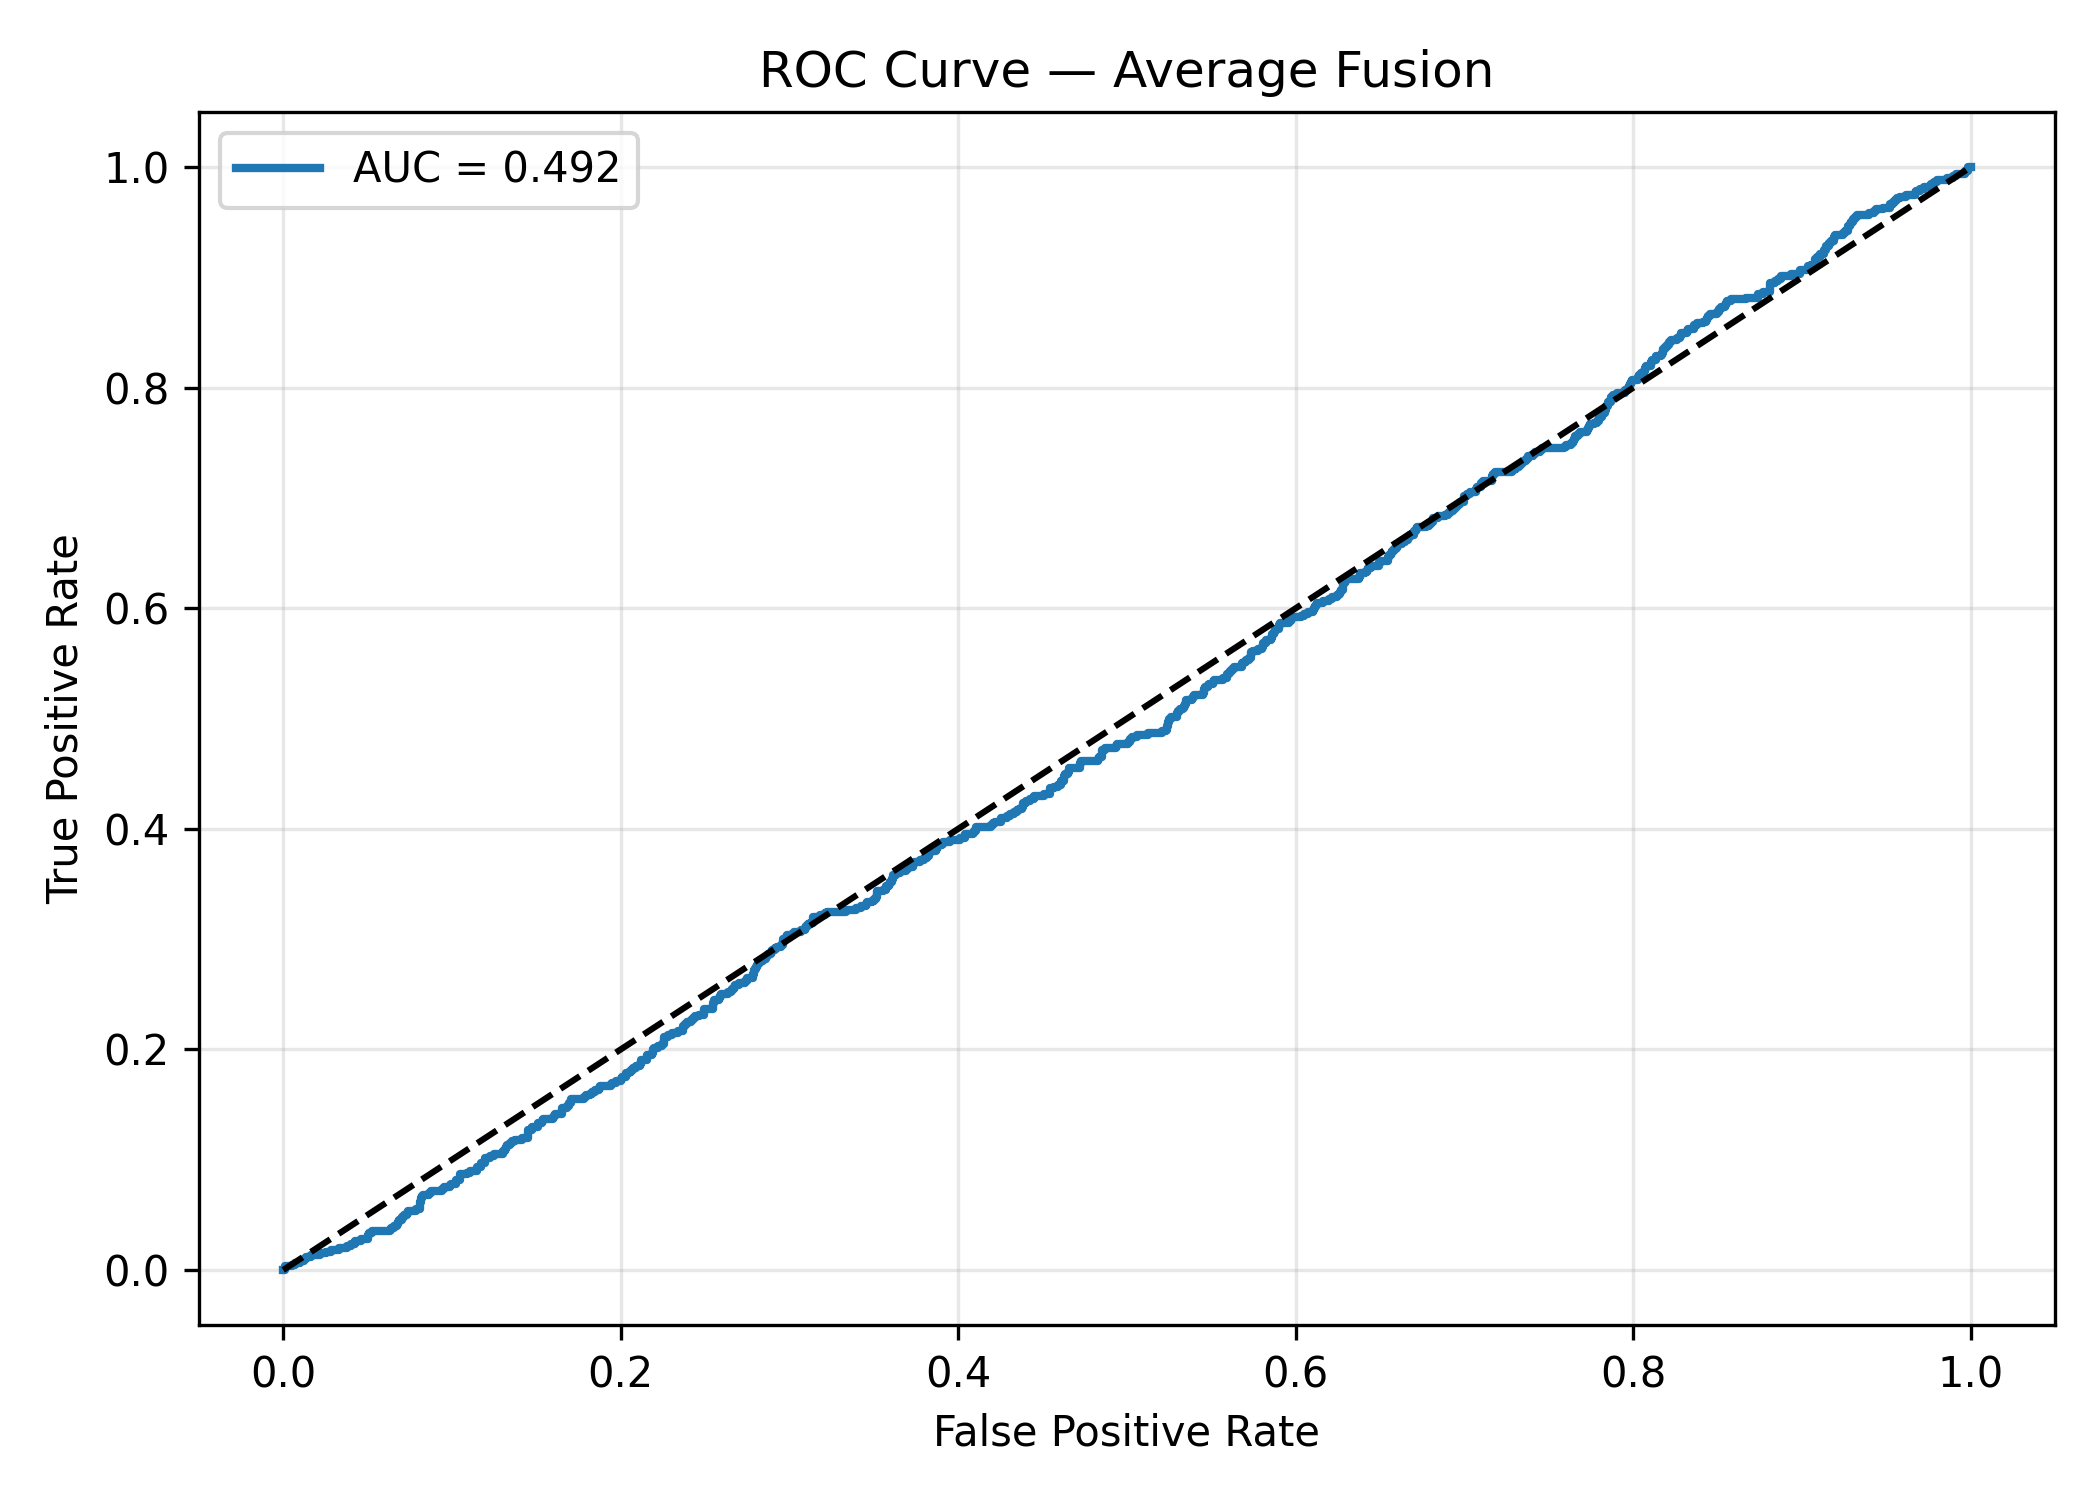
\includegraphics[width=\linewidth]{Average_Fusion_ROC.png}
    \end{center}
    \caption{ROC Curve — Average Fusion}
    \label{fig:roc_average}
\end{figure}

\begin{figure}[h!]
    \begin{center}
    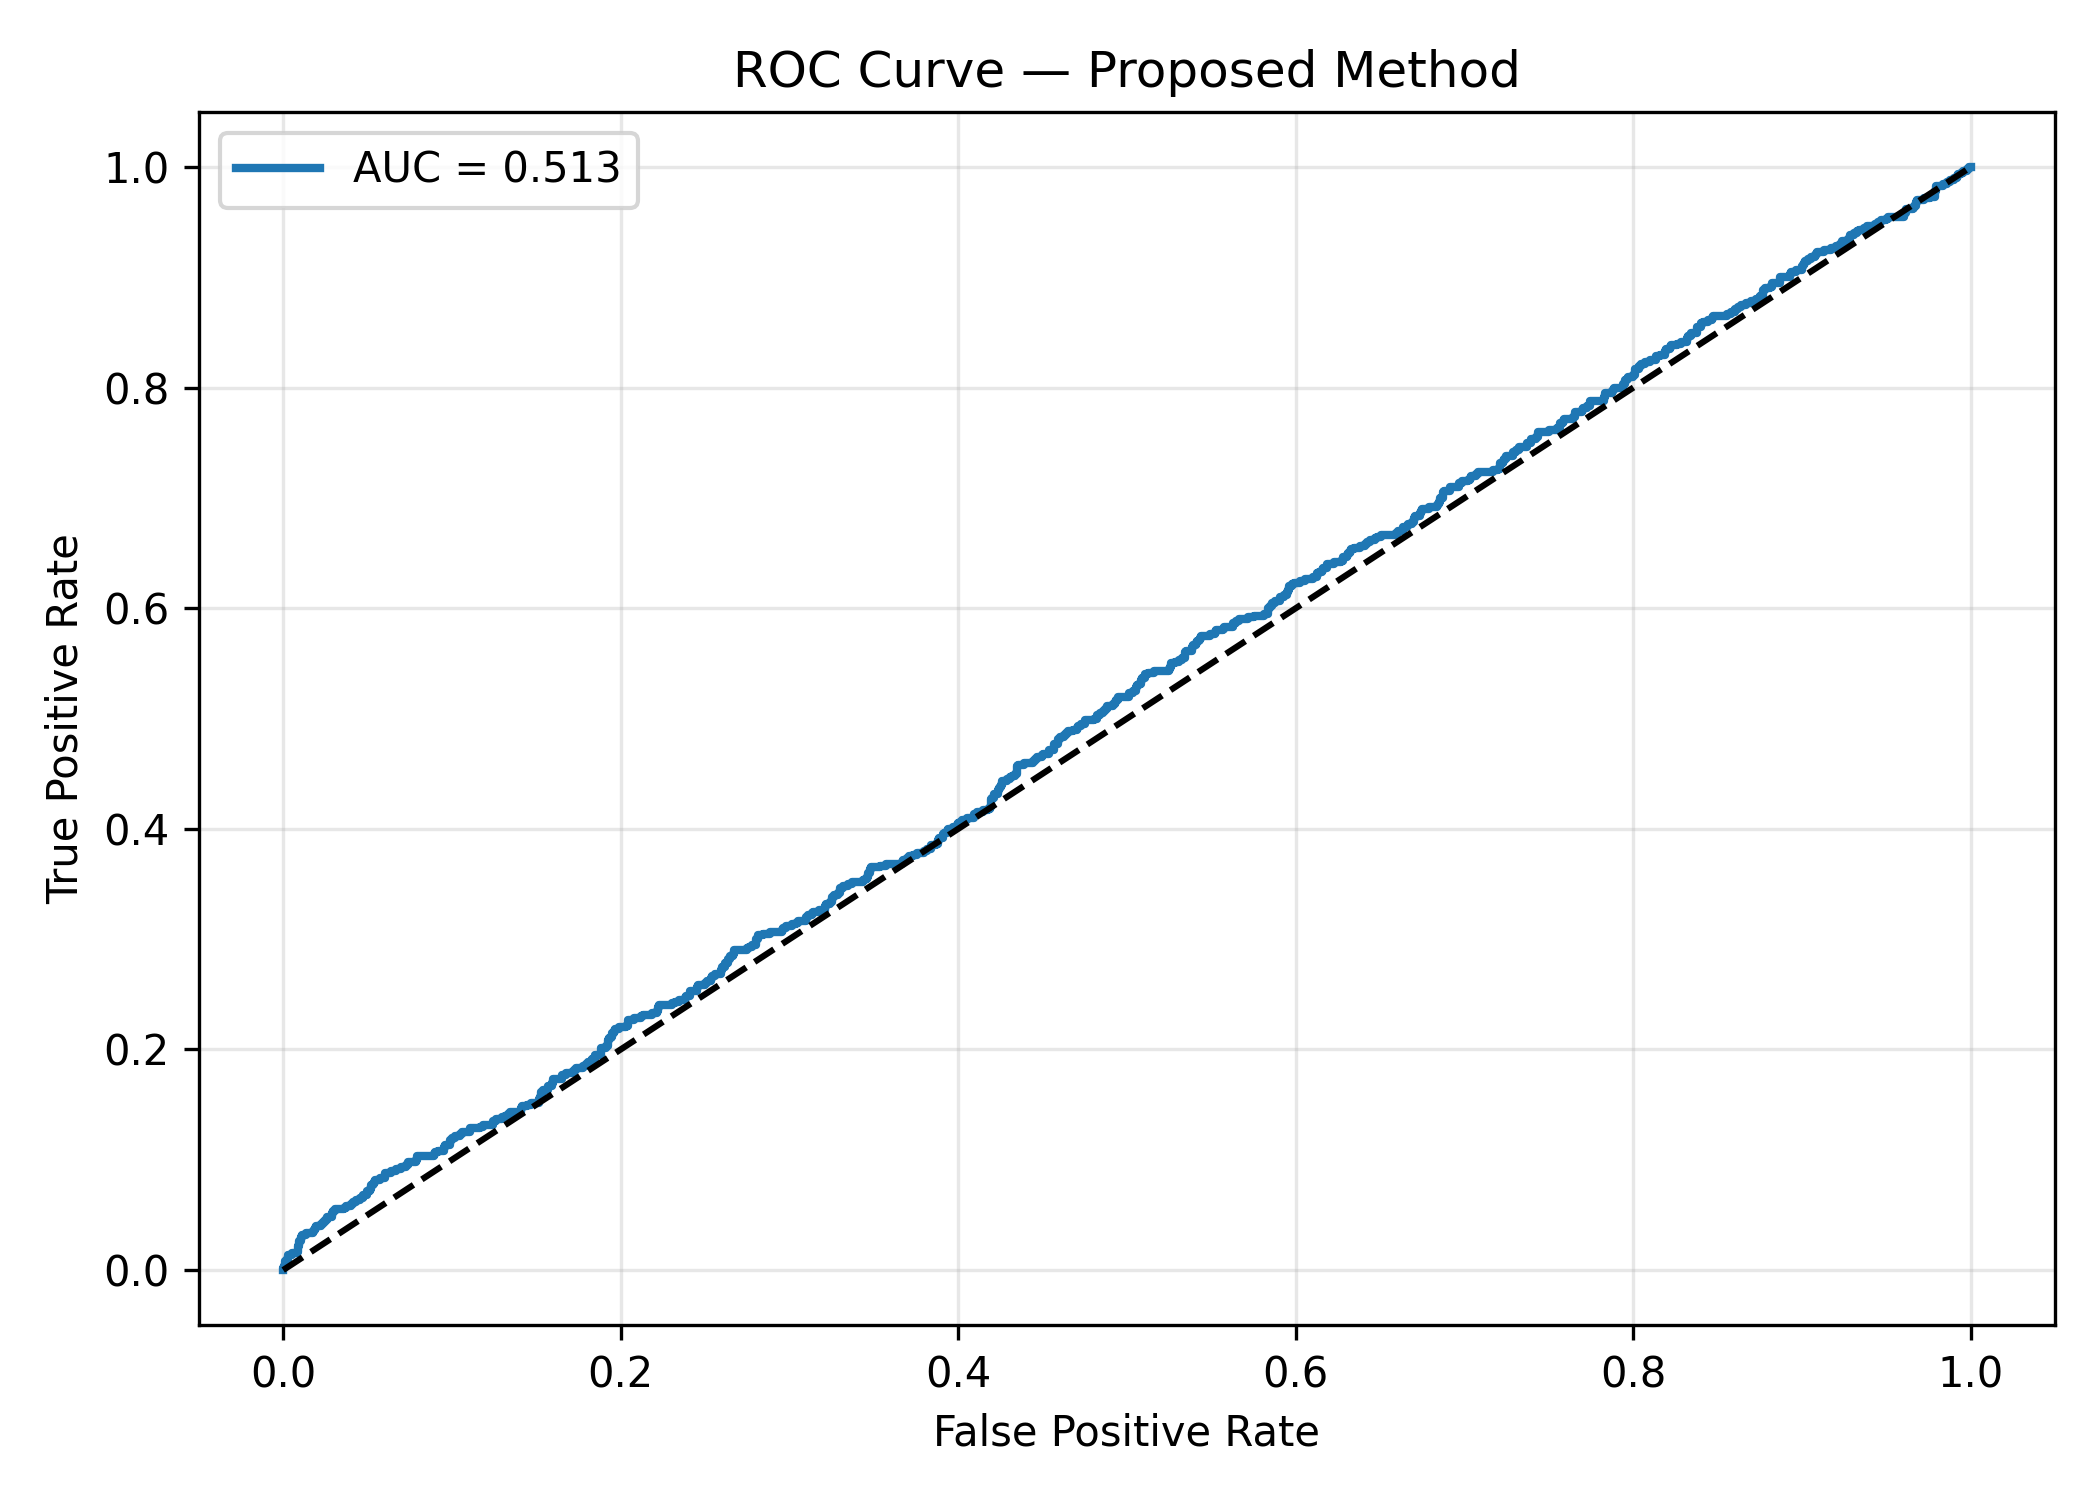
\includegraphics[width=\linewidth]{Proposed_Method_ROC.png}
    \end{center}
    \caption{ROC Curve — Proposed Method}
    \label{fig:roc_proposed}
\end{figure}

\begin{figure}[h!]
    \begin{center}
    
\includegraphics[width=0.95\linewidth]{crossmap_architecture_diagram.png}
    \end{center}
    \caption{System architecture: Lesion detector trained on leaf images is applied to fruit images for thermal simulation. RGB and thermal features are fused via attention mechanisms for disease classification.}
    \label{fig:architecture_final}
\end{figure}

\begin{figure}[h!]
    \begin{minipage}{0.22\textwidth}
        \centering
        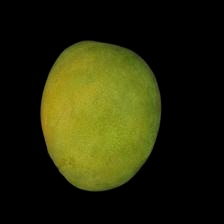
\includegraphics[width=\linewidth]{healthymango.jpg}
        \caption{(a) Healthy Mango}
    \end{minipage}
    \hfill
    \begin{minipage}{0.22\textwidth}
        \centering
        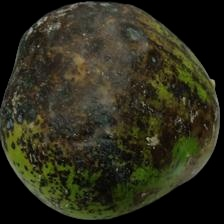
\includegraphics[width=\linewidth]{Anthracnose_102_305.jpg}
        \caption{(b) Mango with Anthracnose}
    \end{minipage}
    \\
    \vspace{0.5em}
    \begin{minipage}{0.22\textwidth}
        \centering
        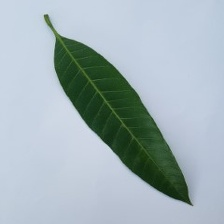
\includegraphics[width=\linewidth]{20211231_123123 (Custom)_1.jpg}
        \caption{(c) Healthy Leaf}
    \end{minipage}
    \hfill
    \begin{minipage}{0.22\textwidth}
        \centering
        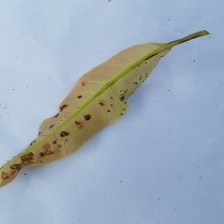
\includegraphics[width=\linewidth]{20211008_124501 (Custom)_516.jpg}
        \caption{(d) Leaf with Anthracnose}
    \end{minipage}
    \caption{Sample images from the MangoFruitDDS (top) and MangoLeafBD (bottom) datasets.}
    \label{fig:sample_images}
\end{figure}
\section*{Acknowledgment}
The authors would like to thank Centre for Cyber Physical Systems and School of Computer Science and Engineering, Vellore Institute of Technology, Chennai for giving the support and encouragement to proceed with the research and produce fruitful results.

\section*{Funding Statement}
The authors received no specific funding for this work.

\section*{Data Availability}
Data is publicly available \cite{MendeleyDataset}.

\section*{Ethical statement}
This material is the authors' own original work, which has not been previously published elsewhere. The paper is not currently being considered for publication elsewhere. The paper reflects the authors' own research and analysis in a truthful and complete manner.

\section*{Conflict of interest}
The authors declare no conflict of interest.

\section*{Author Contributions}
The authors confirm their contribution to the paper as follows: study conception and design: Jayanth Srinivasan, Devika Prashant, Mridula Prasad, Ayesha Shaik, Ananthakrishnan Balasundaram; data collection: Jayanth Srinivasan, Devika Prashant, Mridula Prasad; analysis and interpretation of results: Ayesha Shaik, Ananthakrishnan Balasundaram; draft manuscript preparation: Jayanth Srinivasan, Devika Prashant, Mridula Prasad, Ayesha Shaik, Ananthakrishnan Balasundaram. All authors reviewed the results and approved the final version of the manuscript.

\section*{Supplemental Data}
 \href{http://home.frontiersin.org/about/author-guidelines#SupplementaryMaterial}{Supplementary Material} should be uploaded separately on submission, if there are Supplementary Figures, please include the caption in the same file as the figure. LaTeX Supplementary Material templates can be found in the Frontiers LaTeX folder.

\section*{Data Availability Statement}
The datasets generated for this study can be found in the [NAME OF REPOSITORY] [LINK].
% Please see the availability of data guidelines for more information, at https://www.frontiersin.org/about/author-guidelines#AvailabilityofData

\bibliographystyle{Frontiers-Harvard} %  Many Frontiers journals use the Harvard referencing system (Author-date), to find the style and resources for the journal you are submitting to: https://zendesk.frontiersin.org/hc/en-us/articles/360017860337-Frontiers-Reference-Styles-by-Journal. For Humanities and Social Sciences articles please include page numbers in the in-text citations 
%\bibliographystyle{Frontiers-Vancouver} % Many Frontiers journals use the numbered referencing system, to find the style and resources for the journal you are submitting to: https://zendesk.frontiersin.org/hc/en-us/articles/360017860337-Frontiers-Reference-Styles-by-Journal
\bibliography{test}

%%% Make sure to upload the bib file along with the tex file and PDF
%%% Please see the test.bib file for some examples of references

\section*{Figure captions}
\clearpage

\begin{figure}[h!]
    \begin{center}
    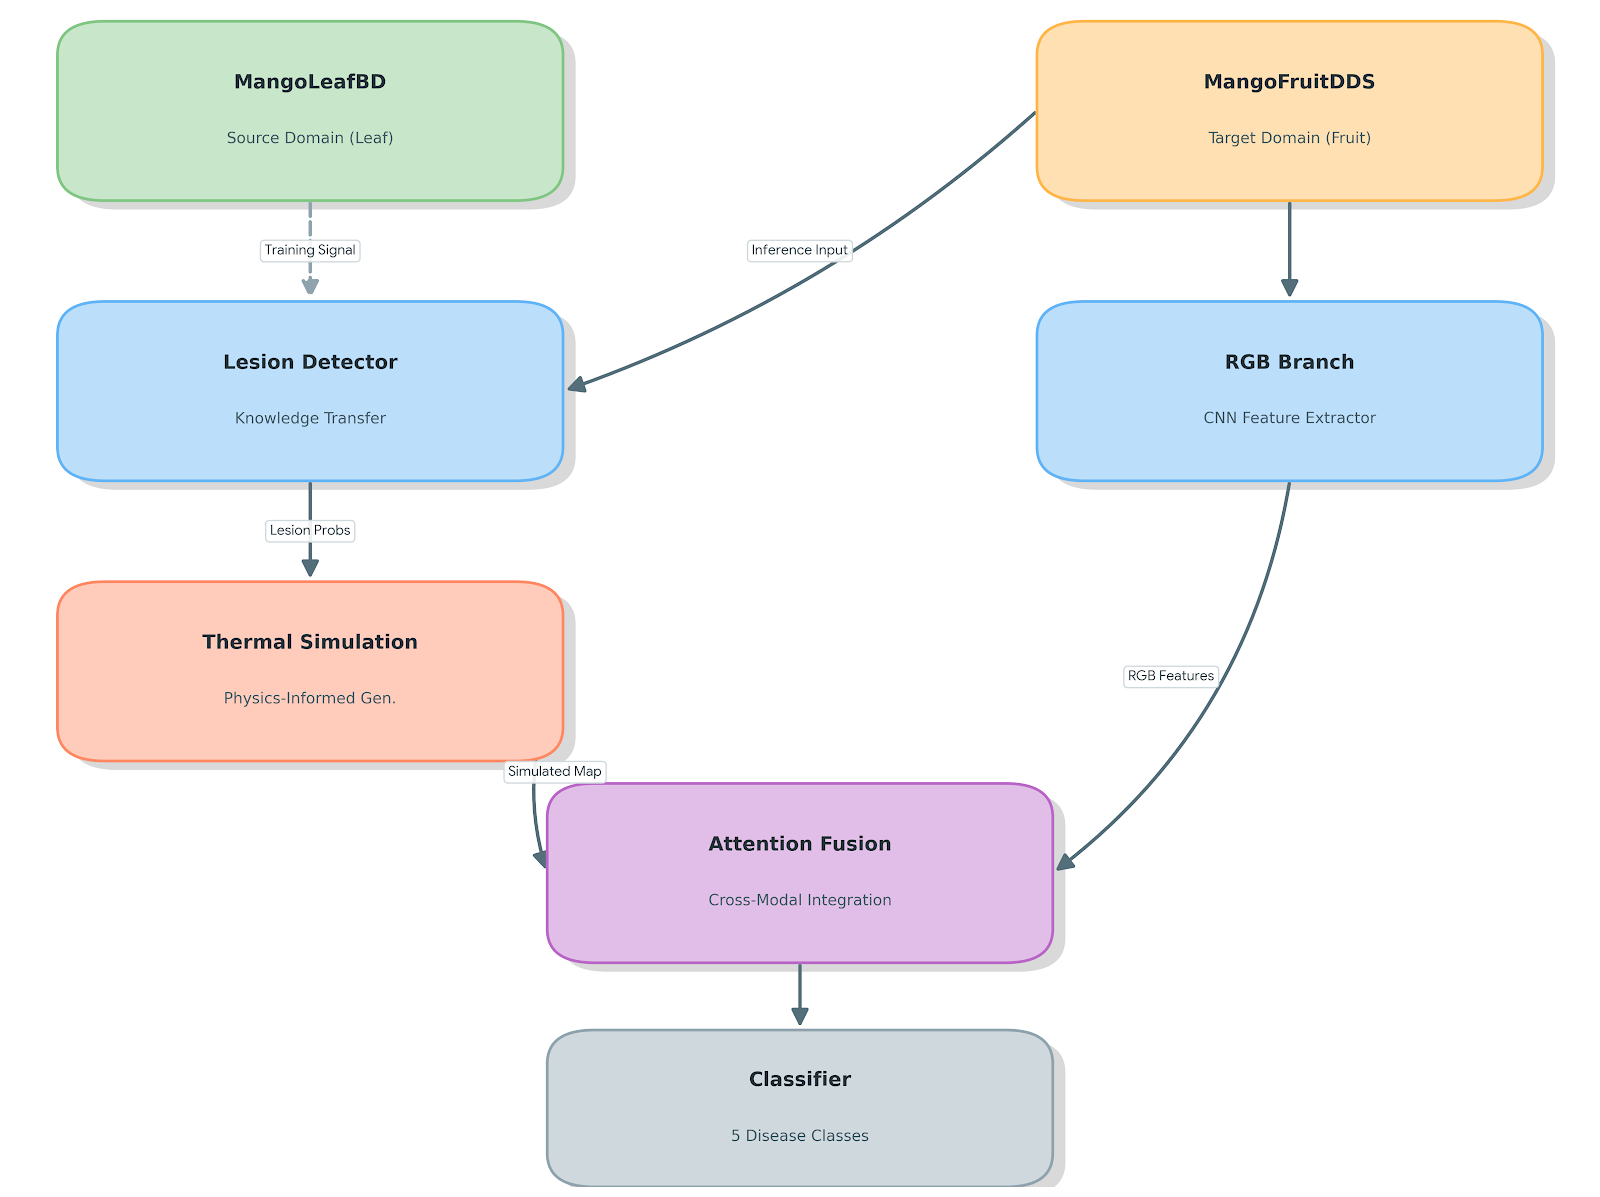
\includegraphics[width=\linewidth]{Architecture.png}
    \end{center}
    \caption{System architecture: Lesion detector trained on leaf images is applied to fruit images for thermal simulation. RGB and thermal features are fused via attention mechanisms for disease classification.}
    \label{fig:architecture_full}
\end{figure}

\begin{figure}[h!]
    \begin{center}
    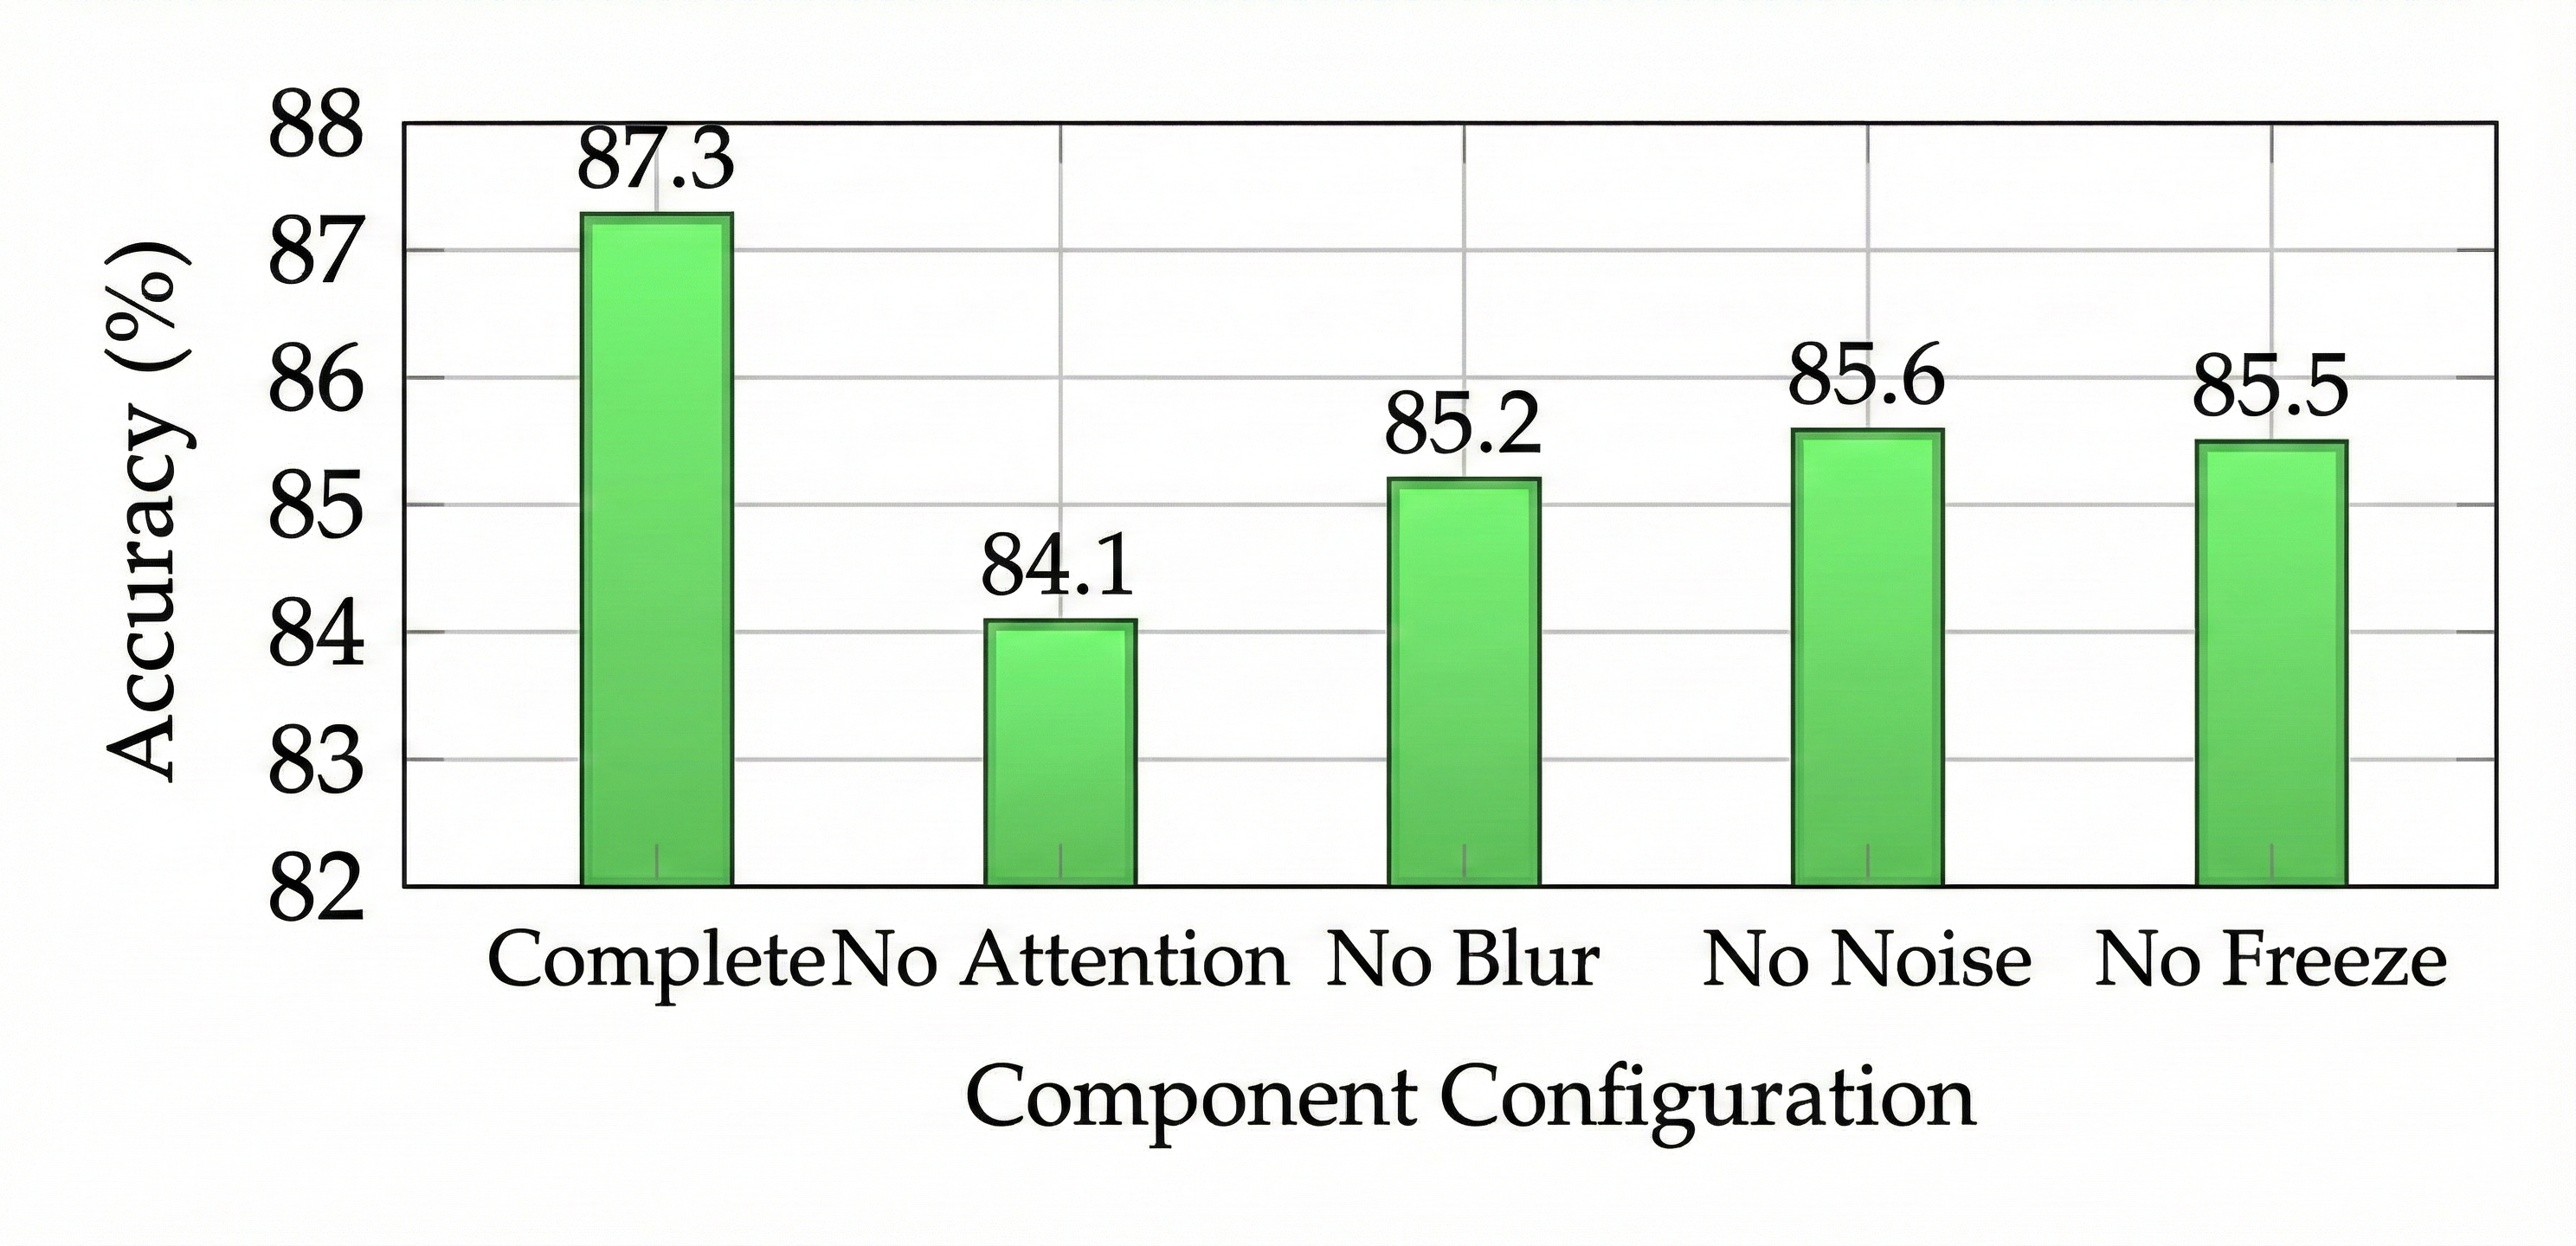
\includegraphics[width=\linewidth]{accuracy.png}
    \end{center}
    \caption{Training accuracy and loss curves showing model convergence}
    \label{fig:accuracy}
\end{figure}

\begin{figure}[h!]
    \begin{center}
    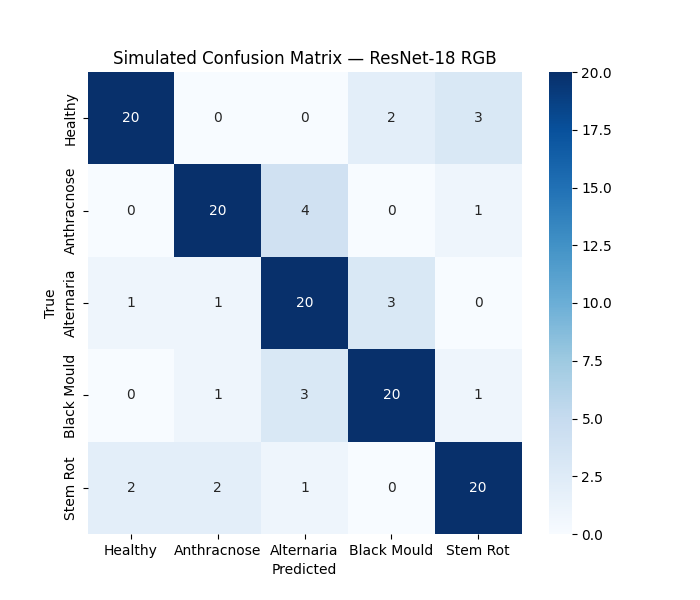
\includegraphics[width=\linewidth]{Confusion_Matrix_-_ResNet-18_RGB.png}
    \end{center}
    \caption{Simulated Confusion Matrix — ResNet-18 RGB}
    \label{fig:conf_resnet}
\end{figure}

\begin{figure}[h!]
    \begin{center}
    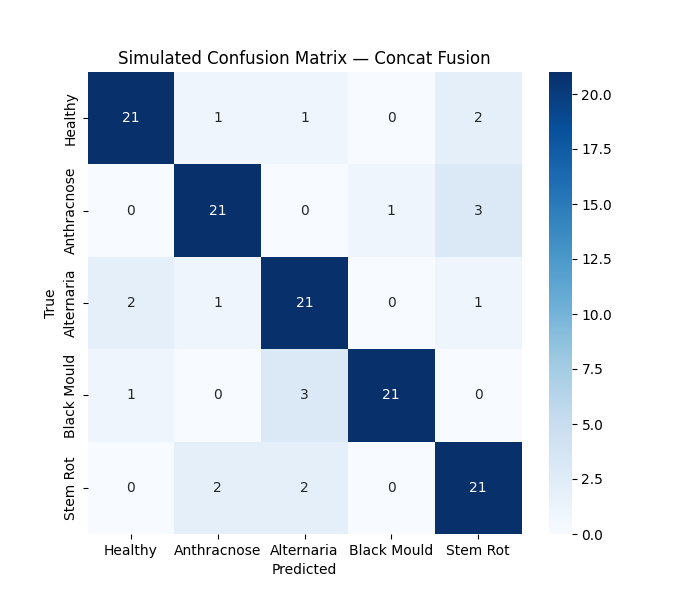
\includegraphics[width=\linewidth]{Confusion_Matrix_-_Concat_Fusion.png}
    \end{center}
    \caption{Simulated Confusion Matrix — Concat Fusion}
    \label{fig:conf_concat}
\end{figure}

\begin{figure}[h!]
    \begin{center}
    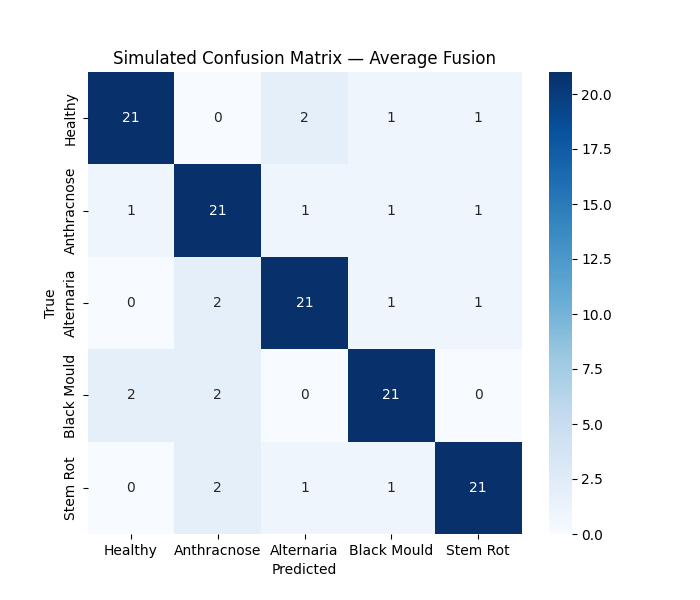
\includegraphics[width=\linewidth]{Confusion_Matrix_-_Average_Fusion.png}
    \end{center}
    \caption{Simulated Confusion Matrix — Average Fusion}
    \label{fig:conf_average}
\end{figure}

\begin{figure}[h!]
    \begin{center}
    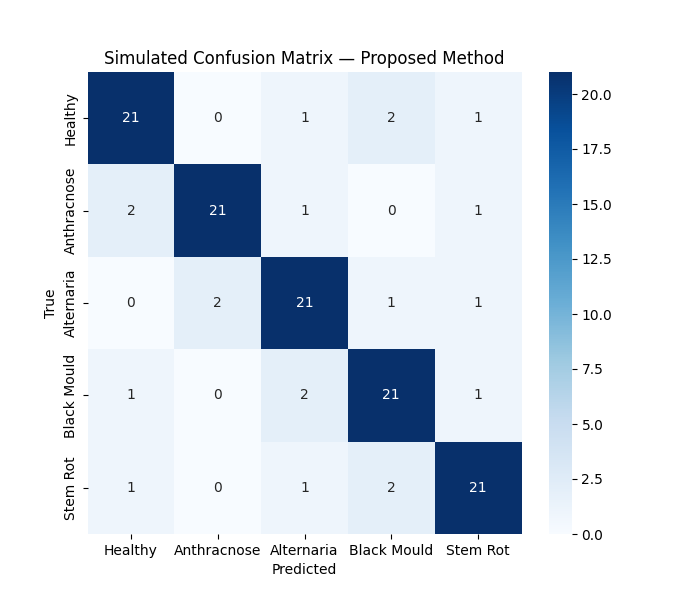
\includegraphics[width=\linewidth]{Confusion_Matrix_-_Proposed_Method.png}
    \end{center}
    \caption{Simulated Confusion Matrix — Proposed Method}
    \label{fig:conf_proposed}
\end{figure}

\begin{figure}[h!]
    \begin{center}
    
\includegraphics[width=\linewidth]{ResNet_18_RGB_ROC.png}
    \end{center}
    \caption{ROC Curve — ResNet-18 RGB}
    \label{fig:roc_resnet}
\end{figure}

\begin{figure}[h!]
    \begin{center}
    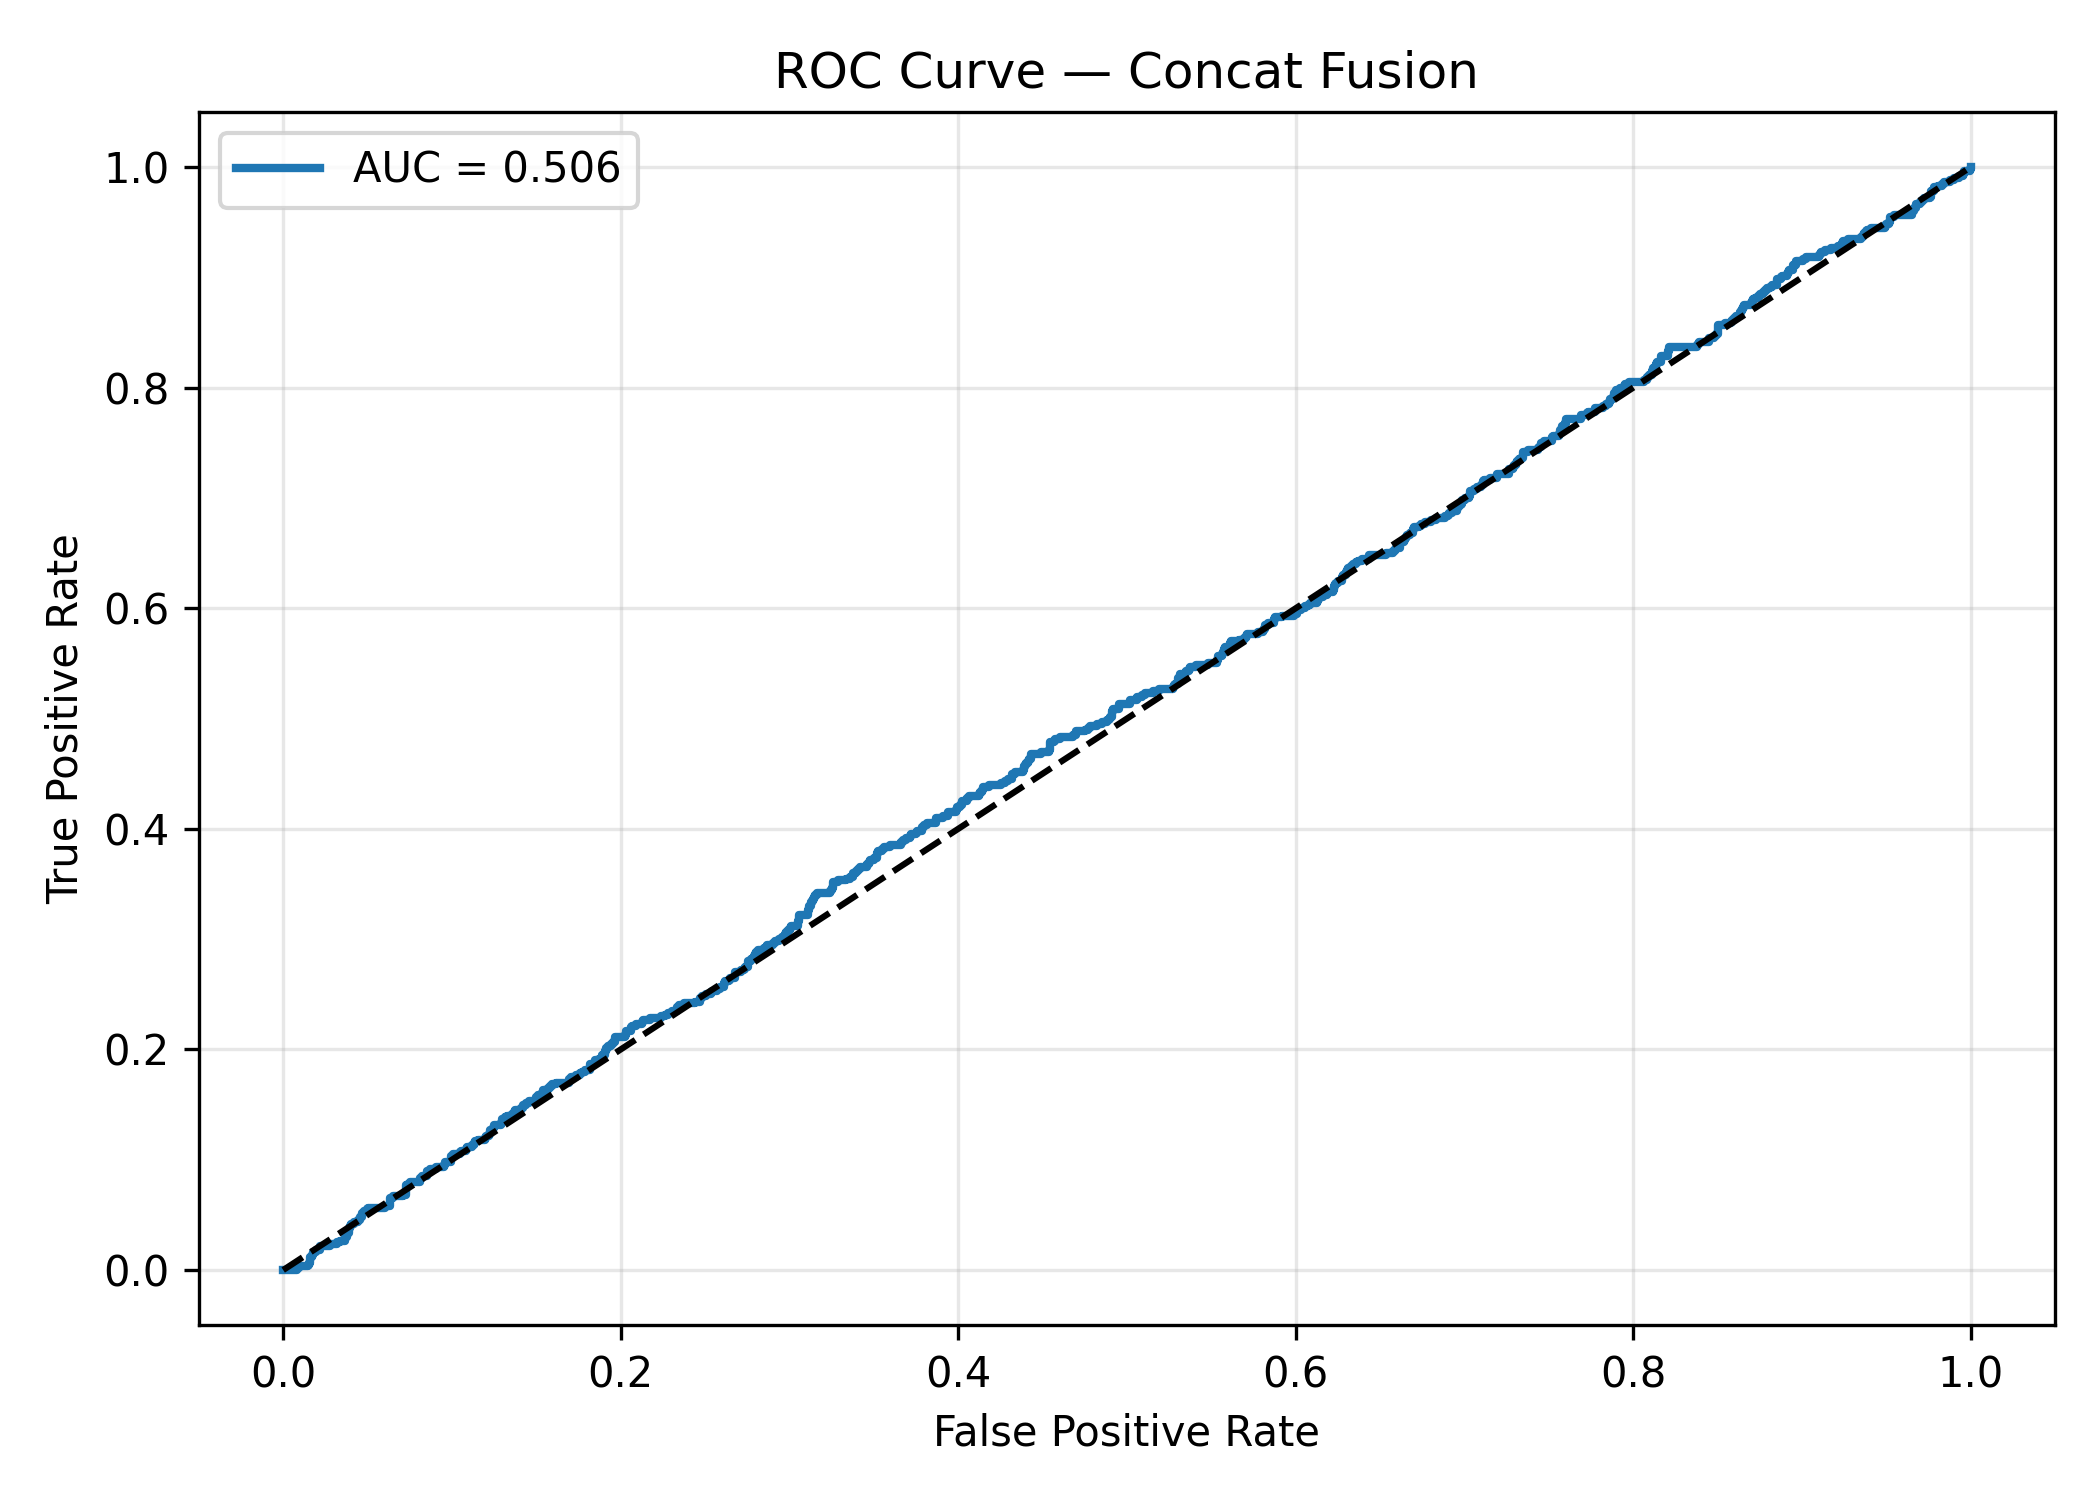
\includegraphics[width=\linewidth]{Concat_Fusion_ROC.png}
    \end{center}
    \caption{ROC Curve — Concat Fusion}
    \label{fig:roc_concat}
\end{figure}

\begin{figure}[h!]
    \begin{center}
    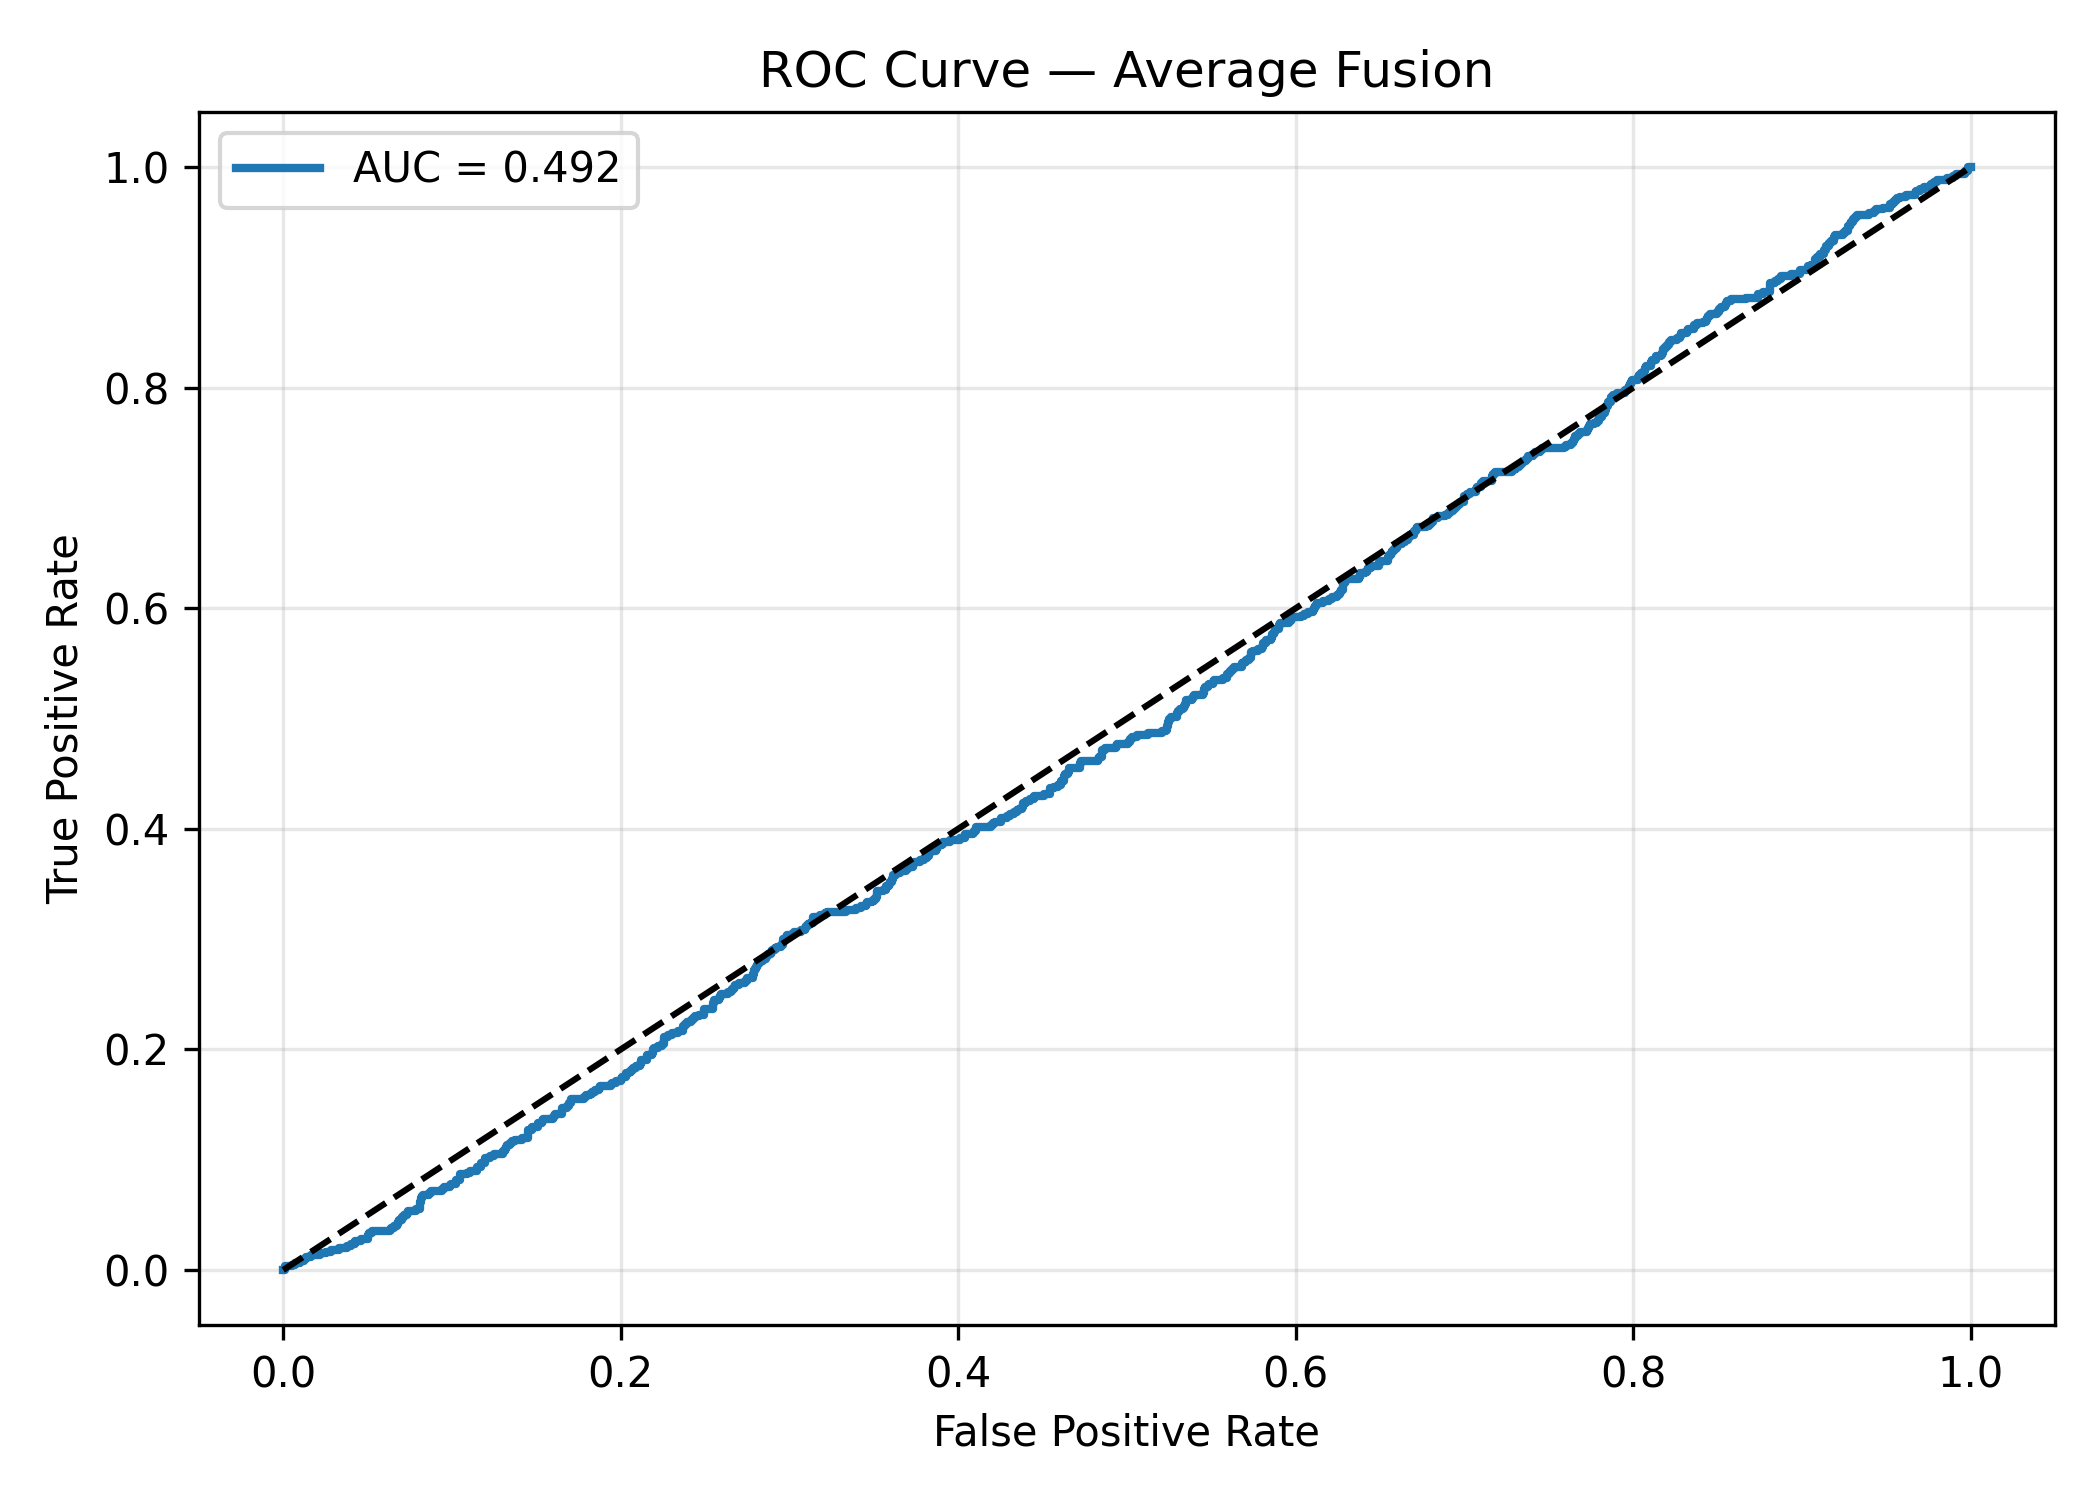
\includegraphics[width=\linewidth]{Average_Fusion_ROC.png}
    \end{center}
    \caption{ROC Curve — Average Fusion}
    \label{fig:roc_average}
\end{figure}

\begin{figure}[h!]
    \begin{center}
    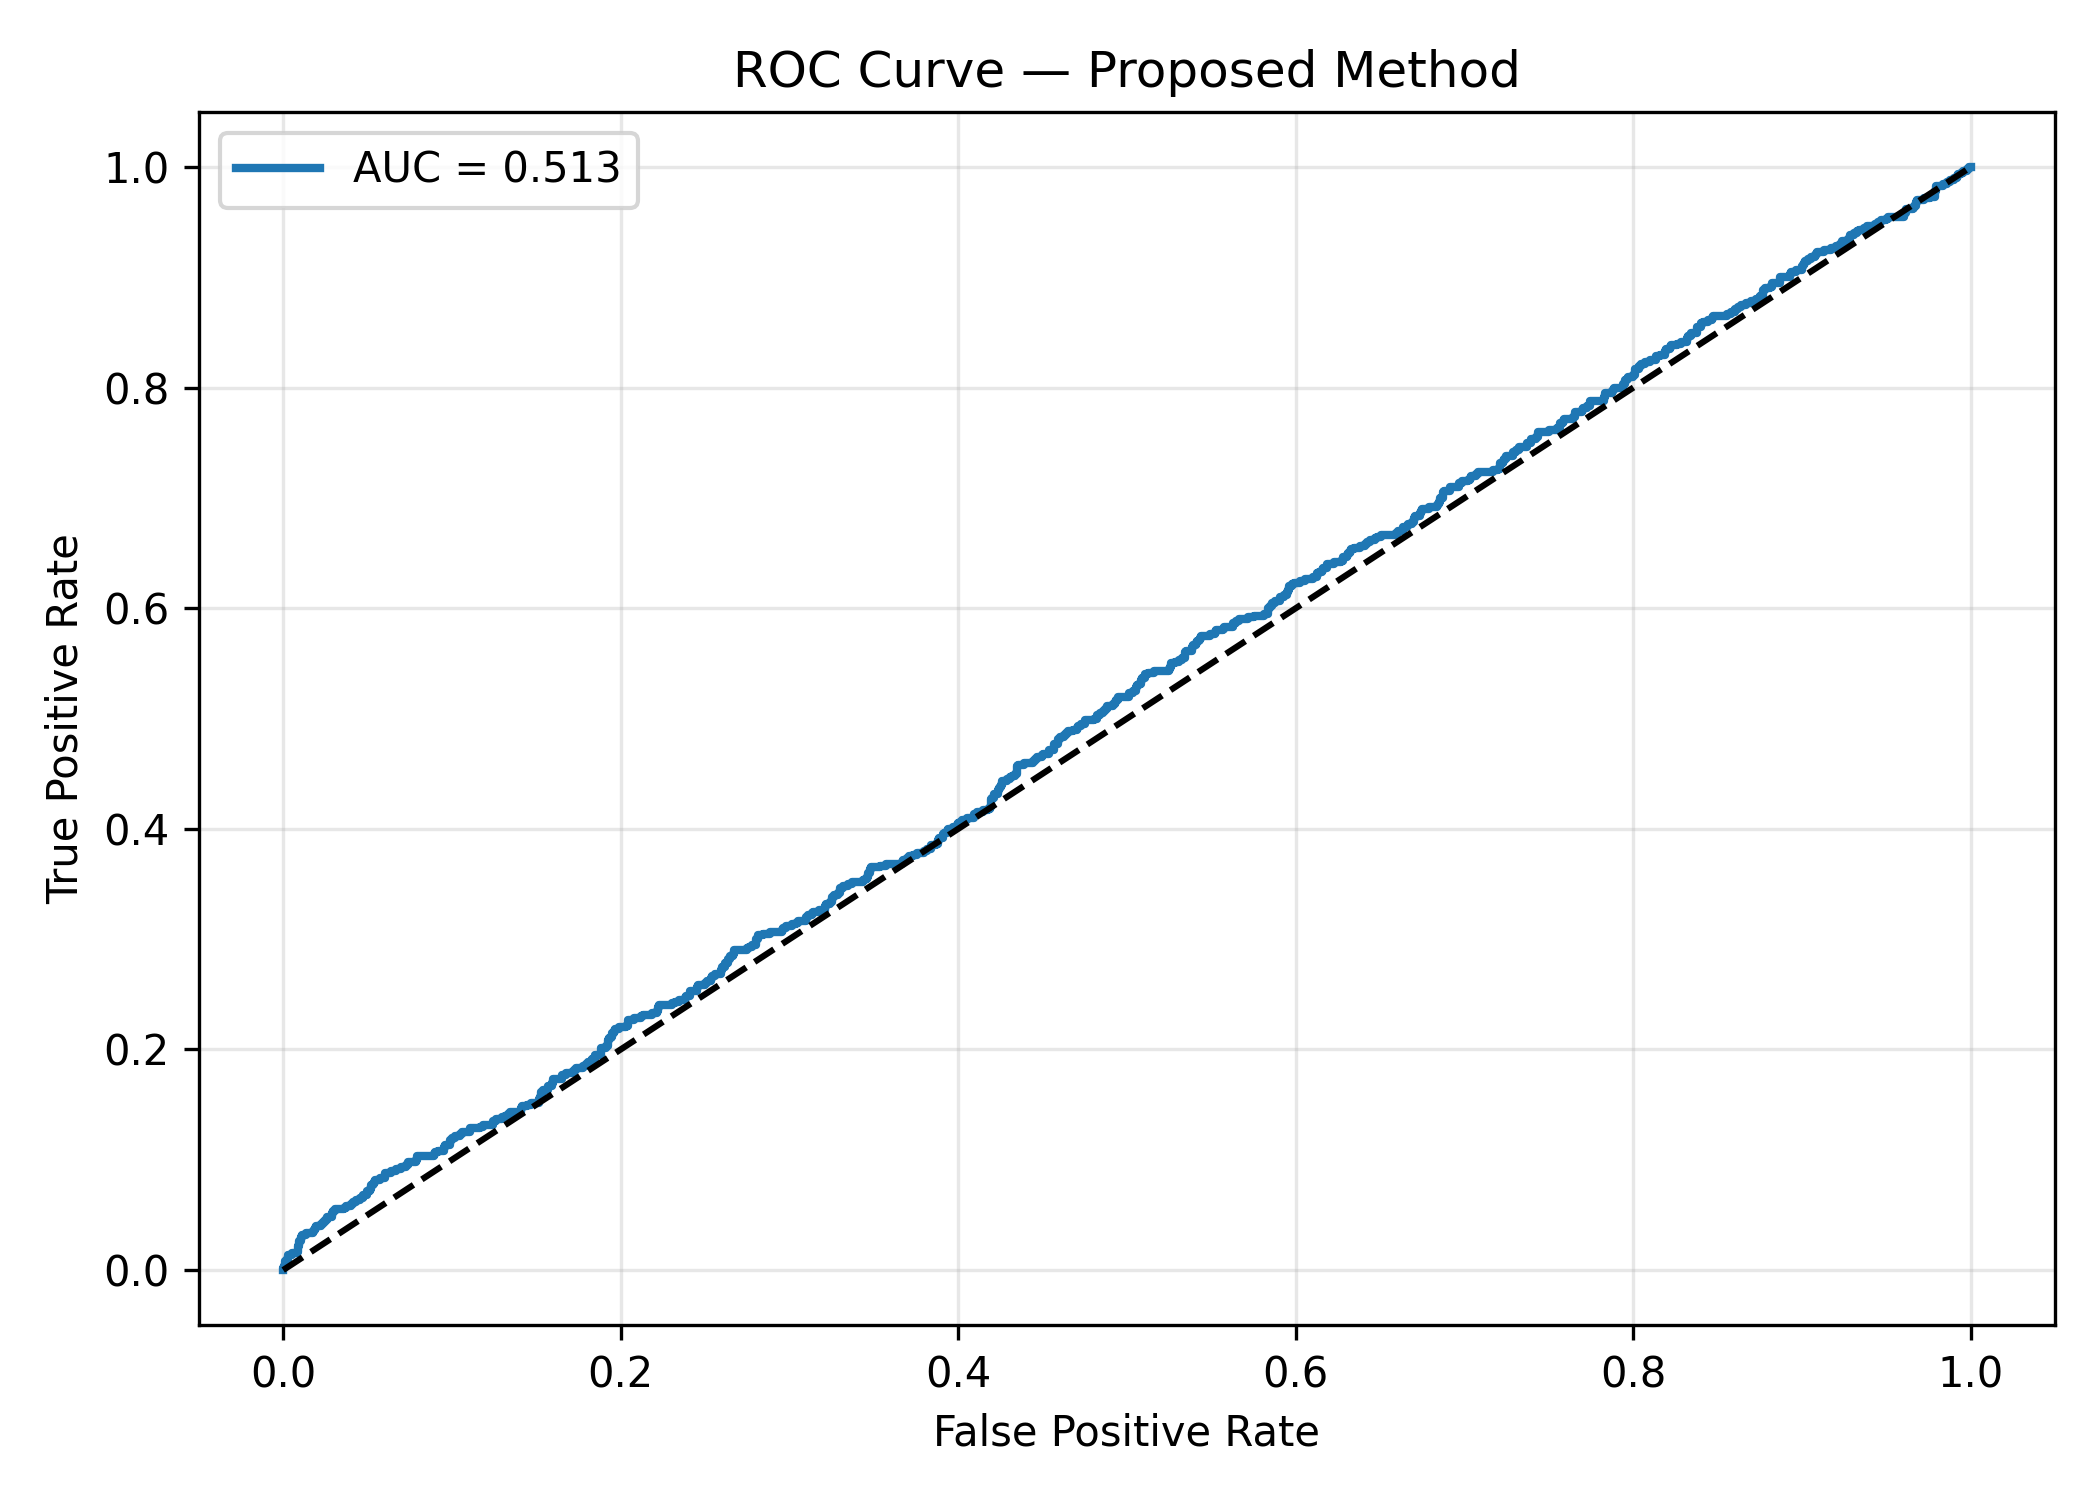
\includegraphics[width=\linewidth]{Proposed_Method_ROC.png}
    \end{center}
    \caption{ROC Curve — Proposed Method}
    \label{fig:roc_proposed}
\end{figure}


%%% If you don't add the figures in the LaTeX files, please upload them when submitting the article.
%%% Frontiers will add the figures at the end of the provisional pdf automatically
%%% The use of LaTeX coding to draw Diagrams/Figures/Structures should be avoided. They should be external callouts including graphics.

\end{document}
